\documentclass[journal,10pt]{IEEEtran}
\usepackage{fontspec}
\usepackage{xeCJK}
\setmainfont{Times New Roman}
\setCJKmainfont[BoldFont=SimHei,ItalicFont=KaiTi]{SimSun}
\setCJKsansfont{Microsoft YaHei}
\setmonofont{Consolas}
\setCJKmonofont{Microsoft YaHei}
\usepackage{amsmath,amssymb,amsfonts}
\usepackage{graphicx}
\graphicspath{{../}{../figures/}{../04_Figures_and_Assets/}}
\usepackage{booktabs,array,multirow,calc,adjustbox}
\usepackage{xcolor}
\usepackage[hidelinks]{hyperref}
\usepackage{xurl}
\usepackage{url}
\urlstyle{same}
\providecommand{\tightlist}{\setlength{\itemsep}{0pt}\setlength{\parskip}{0pt}}
\providecommand{\pandocbounded}[1]{#1}
\providecommand{\passthrough}[1]{#1}
\tracinglostchars=3
\setlength{\emergencystretch}{3em}
\setlength{\textfloatsep}{6pt plus 2pt minus 2pt}
\setlength{\floatsep}{5pt plus 2pt minus 2pt}
\setlength{\intextsep}{5pt plus 2pt minus 2pt}
\renewcommand{\arraystretch}{1.04}
\hyphenation{APAL HGP PPO GraphSAGE}

\title{基于异构图强化学习的飞机脉动装配线联合调度与人员配置}
\author{Xiao~Lu,
        Jiakang~Ai,
        Fei~Qiao,
        Juan~Liu$^*$,
        Lingtao~Chen,
        and~Yumin~Ma%
\thanks{This work was supported by the National Natural Science Foundation of China (Nos. 62133011, 62373288, 62403365, 62273260), and the Open Research Project of the State Key Laboratory of Industrial Control Technology of China (No. ICT2025B28). *Corresponding author}%
\thanks{The authors are with the College of Electronics and Information Engineering, Tongji University, Shanghai, China (e-mail: luxiao@tongji.edu.cn; aijiakang@tongji.edu.cn; fqiao@tongji.edu.cn; juanliu0720@tongji.edu.cn; chenlingtao@tongji.edu.cn; ymma@tongji.edu.cn).}%
}
\markboth{}{Lu \MakeLowercase{\textit{et al.}}: 基于异构图强化学习的飞机脉动装配线联合调度与人员配置}

\begin{document}
\maketitle

\begin{abstract}
飞机脉动装配线（Aircraft Pulsating Assembly Line, APAL）的作业安排涉及工艺前序、站位并发容量、多技能工人和多人协作团队等多资源强耦合约束。工序分站与人员配置相互影响，而具体工人团队的组合选择进一步引发了动作空间爆炸。针对这一问题，本文提出异构图与自回归指针相结合的强化学习联合调度方法 HGP-PPO。首先，将周期作业模板的构造形式化为事件驱动的序贯马尔可夫决策过程（MDP），使用工序、站位、工人和技能四类节点及其拓扑关系联合描述工艺结构与动态资源状态。其次，设计工序---站位---工人的三级条件自回归解码机制，逐步选择工序、物理站位和给定人数的具体工人团队，并通过动态动作掩码与确定性前向时间分配引擎严格维护物理模型约束。工人的站位归属随首次任务指派内生确定并在初始排程中保持固定，有效协调人员配置与各站位动态负荷。在此基础上，通过扩展基准计划与扰动特征并在扰动环境中微调迁移，将该架构适配于物料就绪延误下的周期模板预测---反应式稳定性重调度。基于真实工厂工艺数据构建的四组测试实例包含 Medium（283 道物理工序）、Large（680）、Industrial-I（2,338）与 Industrial-II（3,182）；同一锁定策略在同数据族内无需针对特定实例微调即可生成 100\% 合法的可行排程，外推至近 4 倍训练规模的大实例 Industrial-II 时表现出稳健的解质量，四规模平均完工跨度较适配基线 L2D-PPO-APAL 降低 2.22\%。在 36 个配对物料延误场景中，重调度模型保持 100\% 的排程合法率，平均综合目标值较 L2D-PPO-APAL 和 StabilityAwareRepair 分别降低 7.00\% 和 3.01\%，且在超大规模 Industrial-II 实例下单场景端到端修复仅需约 2 分钟（123.60~s），较元启发式搜索算法展现出超过 30 倍的在线计算扩展性优势。实证结果表明，该方法能够在 APAL 复杂多资源约束下有效协调作业与人员配置，并兼顾计划重调度的完工效率、扰动稳定性与工业级在线实时响应能力。
\end{abstract}

\begin{IEEEkeywords}
飞机脉动装配线，联合调度，人员配置，异构图神经网络，近端策略优化，事件驱动 MDP，稳定性重调度
\end{IEEEkeywords}

\section{引言}\label{sec:introduction}

飞机总装是飞机制造过程的最后关键阶段，涵盖大部件对接、管路敷设、发动机安装、机载系统集成和功能测试等大量复杂作业。相较于自动化批量流水线，飞机总装面向大型复杂装备，具有工艺链长、前序关系密集、单项工时大、作业空间受限以及多工种人工协作程度高等典型特征\cite{fang2021, bao2023, wang2024}。为在重复生产中提高流程化和节拍化水平，现代航空制造业广泛采用飞机脉动装配线（APAL）。APAL 将总装区域划分为若干物理站位，多架在制飞机在流水线上呈脉动节奏依次推进：在一个脉动周期内，各飞机停留在固定站位完成既定工序；周期结束后，所有站位上的在制飞机同步向下游站位转移，直至全部装配完毕\cite{lu2019}。

这种脉动生产组织使局部工序延误具有整线约束效应。全线移站受各站位中耗时最长的``瓶颈站位''严格制约；任一站位因任务分配失衡、技能人员匮乏或站内空间冲突而滞后，都将导致整条装配线停滞等待。因此，合理协调工序分站、站内并行次序与多类关键资源，是实现 APAL 高效平稳运行的核心\cite{becker2006, boysen2007, bao2023}。

在工程实际中，APAL 排程面临多维资源的强耦合联合决策：调度器需要为每道工序同步确定执行顺序、物理站位以及满足技能与人数要求的具体工人团队。若在排程前预先将人员固定到各站位，极易在任务负荷未明前导致人员能力与站位需求严重失衡。因此，工人的站位归属应当在排程构造过程中，随首次入选某站位任务而内生形成。这一机制使团队选择具有持续影响：当前指派不仅决定工序的加工时间与资源占用，还会确定未绑定工人的站位归属，从而影响后续工序的人员可选范围。因此，当前工序的执行效率与后续站位的技能资源需求需要在同一决策过程中协调。这一联合决策面临显著难题：首先，工序、站位、工人和技能具有异质拓扑关系，排程状态高度动态；其次，每道工序需从多名多技能候选人中指派多人团队，形成规模为 $\binom{n_i}{q_i}$ 的离散组合选人空间；再次，每次子决策均会实时改变后续可选资源与可行域。更进一步，在遭遇物料到货延误等制造现场扰动时，生产系统需在计划冻结边界处严格继承既定计划与工人---站位绑定，对后续周期作业模板进行重新平衡与稳定性修复，以在恢复物理可行性的同时兼顾完工节拍与计划扰动惩罚\cite{vieira2003, hu2024}。

\begin{figure*}[!t]
\centering
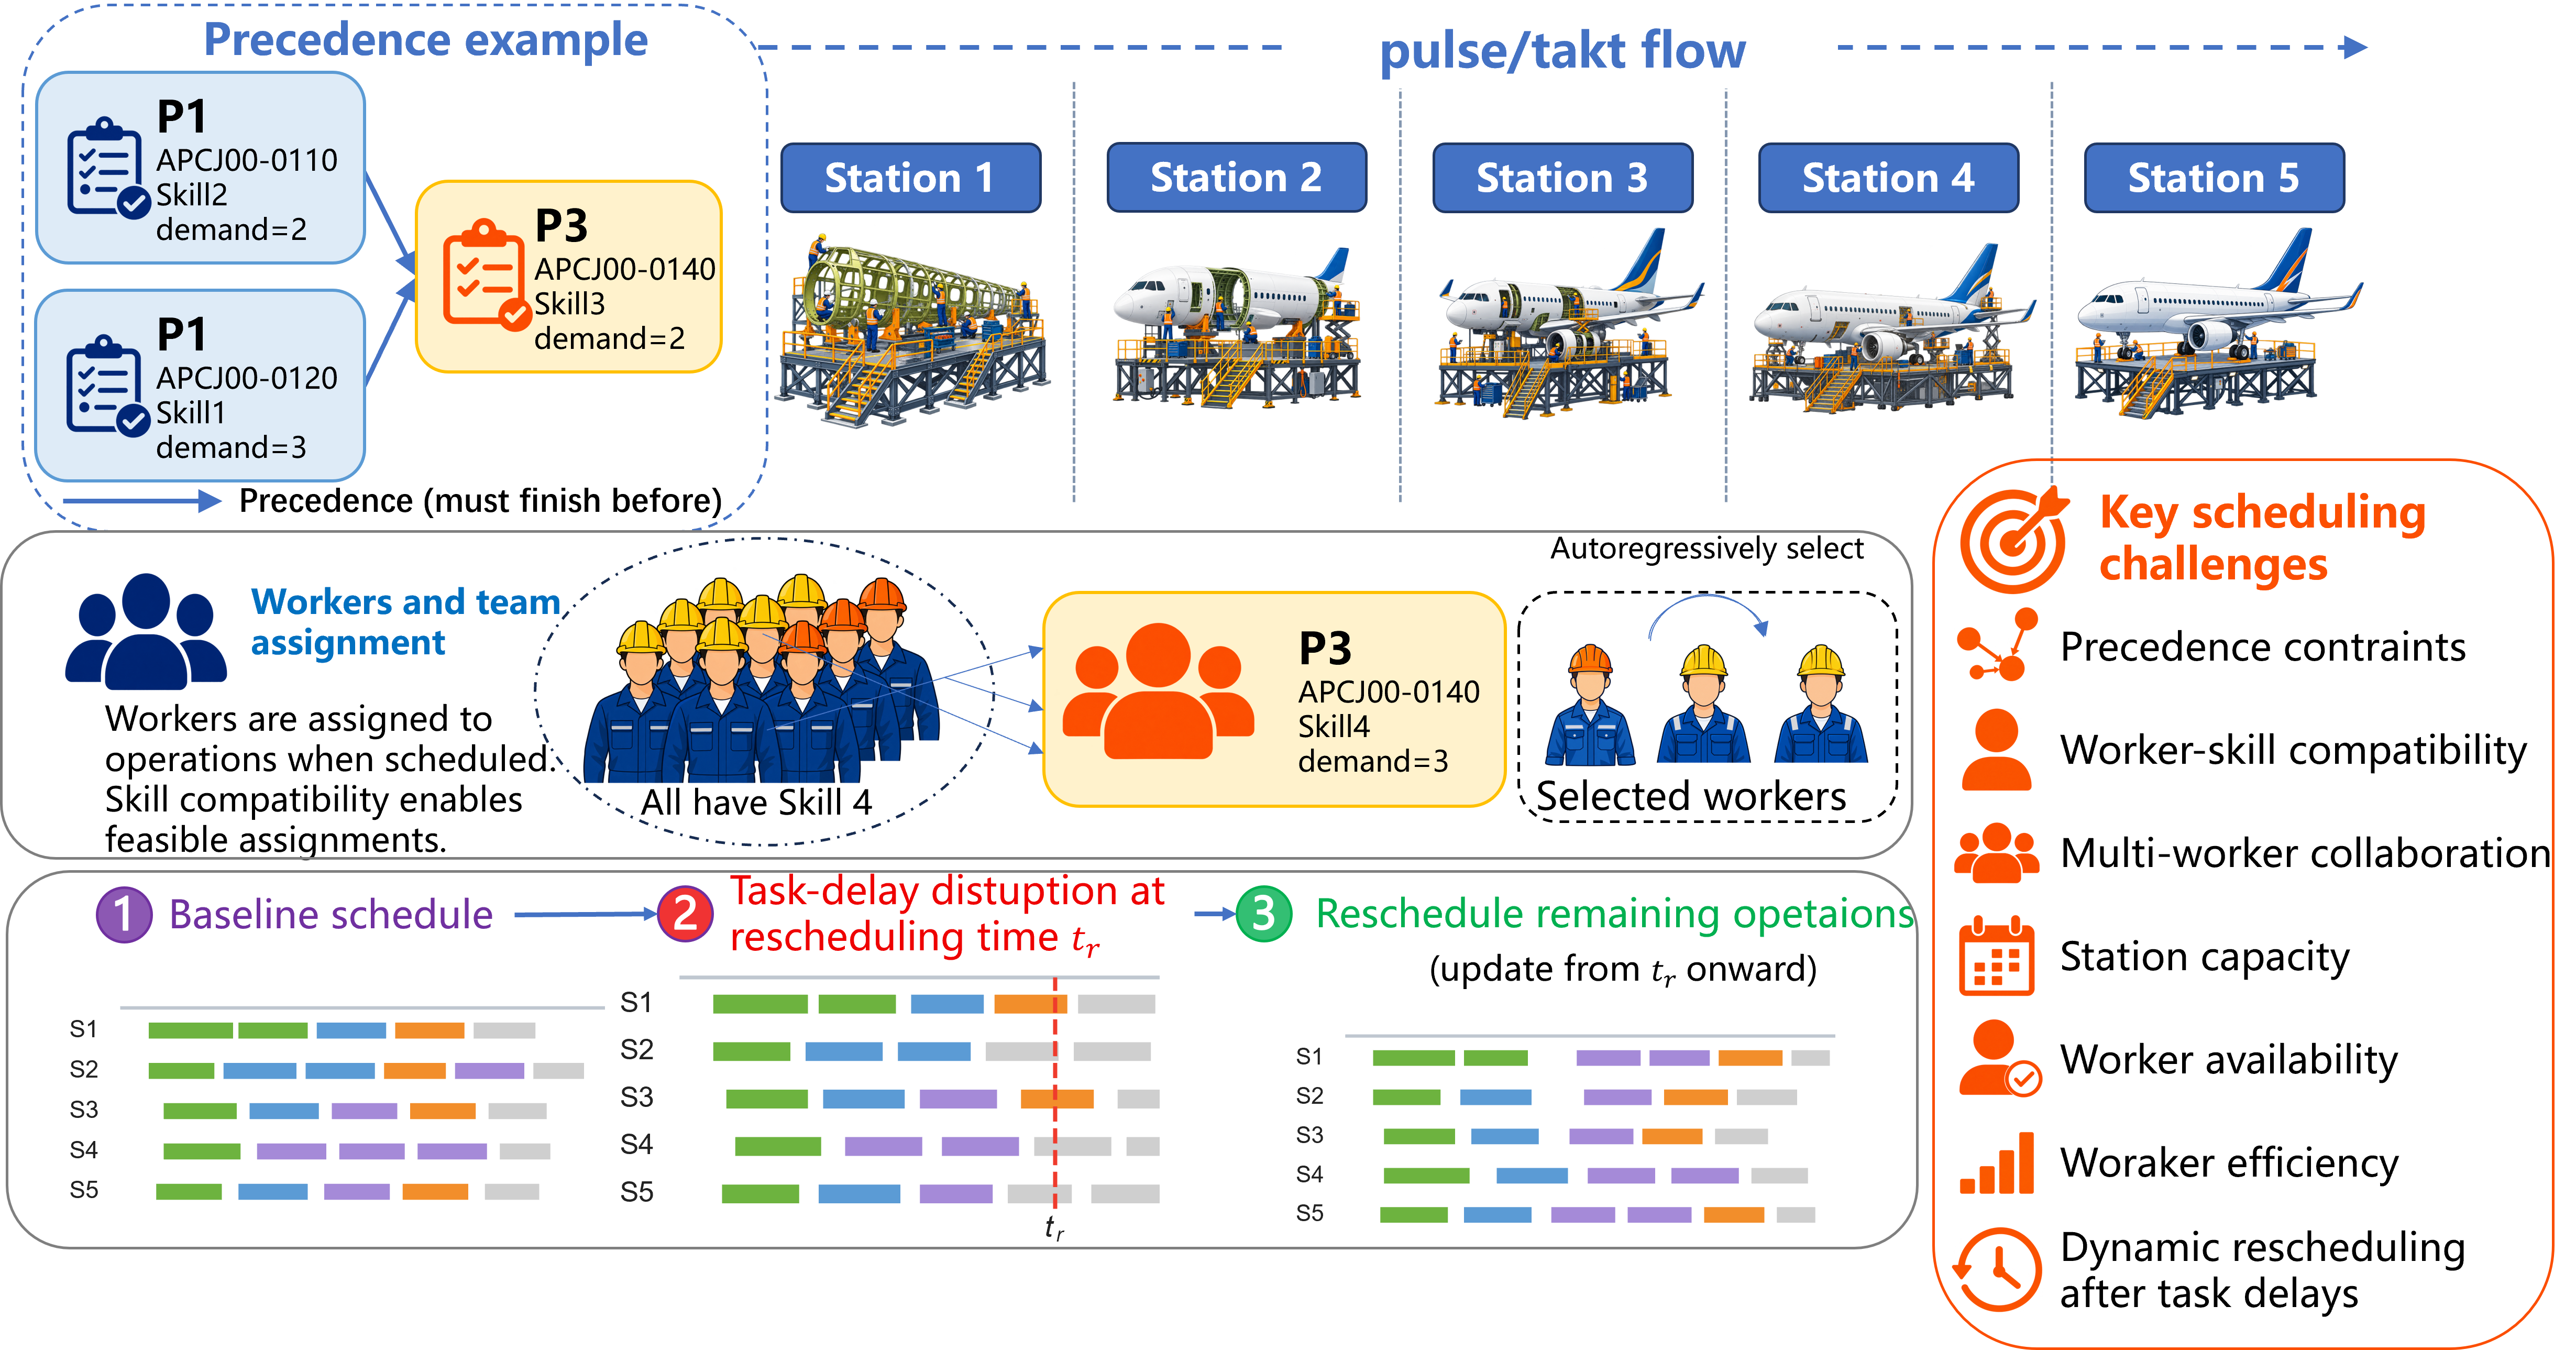
\includegraphics[width=\textwidth,height=0.22\textheight,keepaspectratio]{figures/fig1.png}
\vspace{2pt}
\parbox{\textwidth}{\footnotesize \textbf{图 1　飞机脉动装配线周期作业排程与稳定性重调度问题示意。} 飞机在五个物理站位间呈脉动节奏推进。周期作业模板需联合确定工序的前序执行关系、所属站位及满足技能与人数要求的具体工人团队。发生物料就绪延误后，系统在计划冻结边界 $\tau^r$ 处锁定既定条目并继承工人站位绑定，对后续工序开展稳定性重调度。}
\end{figure*}

针对飞机脉动装配线中作业安排与人员配置相互制约的问题，本文提出 HGP-PPO 联合调度框架，主要贡献如下：
\begin{enumerate}
\item \textbf{面向内生人员配置的联合调度建模。}建立同时考虑工艺前序、站位并发容量和多技能多人协作的 APAL 周期作业模板模型，将工序分站、具体团队选择与工人站位归属纳入统一的序贯构造过程。通过首次指派形成的持续性站位绑定，显式刻画当前团队选择对后续人员可用性的影响，实现作业安排与站位人员配置的协同确定。
\item \textbf{面向工艺与技能供需耦合的异构图表示。}构建由工序、站位、工人和技能组成的异构图，联合表示工艺依赖、技能供需及动态指派关系。通过关系特定的注意力编码，为工序分站与团队构造提供共享的状态表示，使策略能够结合任务结构与人员资源状态进行联合决策。
\item \textbf{融合团队状态与技能稀缺度的自回归联合解码。}设计工序---站位---工人的条件指针机制，将固定人数团队的组合选择分解为逐成员决策，并结合部分团队表示、试探完工特征与额外技能边际稀缺度，对候选成员进行条件评分。该机制避免显式枚举完整团队，并通过动态掩码与前向时间分配执行所建模型的约束。
\end{enumerate}

围绕初始调度与物料延误重调度，本文分别评价上述框架的联合排程能力与计划修复能力。初始调度采用同一锁定策略，在包含 Medium（283 道物理工序）、Large（680）、Industrial-I（2,338）与 Industrial-II（3,182）的四个真实工厂测试实例上开展无需微调的跨规模评价，并通过人员预配置、图表示及决策架构对比分析整体设计的作用。在此基础上，通过扩展基准计划与扰动特征并继续微调，将框架适配于继承冻结作业和既有工人站位绑定的周期模板稳定性重调度，在 36 个配对扰动场景中评价排程合法性、完工效率、计划偏离与在线求解时间。上述实验共同考察所提方法在所研究 APAL 数据族内的跨规模可用性，以及从初始模板构造到受扰模板修复的适用能力。

本文其余章节安排如下：第二章评述相关研究；第三章建立 APAL 联合调度与重调度数学模型；第四章阐明 HGP-PPO 算法架构与决策机制；第五章报告多尺度实验与消融对比结果；第六章给出结论与局限性讨论。

\section{相关工作}\label{sec:related_work}

\subsection{飞机装配排程与多资源人员配置}\label{sec:rel_apal}

装配线平衡与调度（ALBP/SALBP/GALBP）形成了工序分站与负荷平衡的经典运筹学体系\cite{becker2006, boysen2007, battaia2013}。近年来，针对飞机总装大部件对接与密集装配等复杂工况，学者们进一步将资源与人员约束纳入模型。Bao 等\cite{bao2023, bao2023b}联合优化了工序分站平衡与多类资源配置，但主要采用分阶段启发式搜索；P. Fang 等\cite{fang2021flexible}和 D. Wang 等\cite{wang2024}研究了多阶段装配中跨站移动的柔性人员配置；Liu 等\cite{liu2025}及 Wen 等\cite{wen2026}分别在站内派工层面探讨了多技能工人和熟练工等级配置。上述研究证明了多资源约束对装配周期的显著影响，但其决策大多发生在工序分站之后，或仅优化人员流动数量与资源宏观配置。与之不同，本文面向未提前指定站位、人员尚未绑定的全局场景，在同一决策过程中联合确定工序、物理站位以及满足人数要求的具体工人团队。

\subsection{生产调度中的图强化学习与结构化动作}\label{sec:rel_gnn_rl}

图神经网络通过共享的消息传递机制学习组合优化问题中的结构化表征，已成为车间智能调度的重要工具\cite{cappart2023}。在 JSSP 与 FJSP 领域，基于图的强化学习方法通过编码工序工艺依赖与机器约束来学习派工策略\cite{zhang2020, park2021, wang2024flexible}。在飞机装配领域，课题组前序工作\cite{ai2025}初步验证了图增强策略在 APAL 平衡中的有效性；Wen 等\cite{wen2026b}结合 GIN 与 PPO 求解了包含技能等级与空间容量的装配调度。然而，主流调度强化学习的动作空间大多局限于选择下一道工序或工序---单机器配对。面对多人协作团队的组合选择空间与动态人员站位归属，所提框架通过包含工序、站位、工人和技能的异构图联合表示工艺依赖与技能供需关系，并采用工序---站位---工人自回归解码器构建团队。部分团队状态与技能稀缺度特征指导逐成员选择，并通过动态掩码执行工人技能资质与站位绑定约束。

\subsection{装配线扰动重调度与计划稳定性}\label{sec:rel_resched}

在动态制造环境下，预测---反应式调度提供了事前制定基准方案、事后针对扰动触发调整的标准范式\cite{vieira2003, vonder2007}。面向飞机移动装配中的供应链不确定性，Zhu 等\cite{zhu2021}针对物料延迟调整了未开始作业；Hu 等\cite{hu2024}提出了工时波动下的两阶段逆调度与资源重分配策略；Chen 等\cite{chen2026}进一步利用多智能体强化学习在物料延迟下动态切换派工规则。在飞机脉动装配线中，重调度必须兼顾同步脉动移站机制。本文聚焦物料就绪延误下的计划级周期作业模板二次平衡，严格继承冻结作业与既有工人站位绑定。将基准计划与扰动特征融入联合决策框架并继续训练，以协同平衡完工效率与工序开工时间、站位指派和团队构成的计划偏离。

\section{APAL 联合排程与重调度问题建模}\label{sec:problem}

\subsection{APAL 系统描述、核心假设与符号}\label{sec:problem_desc}

考虑由 5 个固定物理站位组成的飞机脉动装配线（APAL）。装配工艺原始拓扑表示为有向无环图 $G=(\mathcal{O},\mathcal{E})$，工序集合 $\mathcal{O}=\mathcal{O}^{+}\cup\mathcal{O}^{0}$，其中 $\mathcal{O}^{+}$ 表示加工时间大于零的实际物理工序，$\mathcal{O}^{0}$ 表示非执行性工艺结构节点（工时为零，仅用于保留工艺层级关系，下文简称为结构节点）。结构节点不占用物理资源。物理前序关系通过绕过结构节点并保持物理工序间依赖关系导出，构成实际物理工序有向图 $G^+=(\mathcal{O}^+,\mathcal{E}^+)$；工序 $i$ 的物理紧前工序集合记为 $\mathcal{P}(i)$。系统包含多技能工人池 $\mathcal{W}$ 和五类技能集合 $\mathcal{K}$（$|\mathcal{K}|=5$），物理站位集合为 $\mathcal{M}=\{1,\dots,5\}$。每道工序 $i\in\mathcal{O}^{+}$ 具有基础标准持续时间 $p_i^{\mathrm{std}}>0$、所需单一技能类型 $k_i\in\mathcal{K}$ 和固定团队人数 $q_i\in\mathbb{N}^{+}$；每名工人 $w\in\mathcal{W}$ 具备二元技能资格向量 $\mathbf{H}_w=(H_{wk})_{k\in\mathcal{K}}$（其中 $H_{wk}\in\{0,1\}$）和基础效率系数 $\eta_w>0$。除少量初始就位工序外，工序所属站位不预先指定。

本模型采用以下运行假设：
\begin{enumerate}
\item \textit{工序不可抢占（Non-preemptive operations）：} 工序一旦开工，其中途不得中断，所属站位与执行团队在完工前保持不变。
\item \textit{转移与准备时间（Transfer and setup times）：} 工序转移与准备时间已包含在工厂提供的标准工时中。
\item \textit{资源可用性（Resource availability）：} 工人与站位在整个规划周期内保持正常可用，不发生非预期的设备故障或人员缺勤。资源的使用仍严格受限于工人单任务互斥与站位并发容量上限。
\item \textit{工人---站位绑定（Worker--station binding）：} 所有工人初始处于无站位绑定状态。每名工人的站位归属在首次被分配任务时确立，并在该初始排程中保持固定。因此，在该排程内工人不得跨不同站位执行工序。该站位分配在后续重调度中严格继承。
\end{enumerate}

\begin{table}[!t]
\centering
\caption{主要数学符号（Main Mathematical Notation）}
\label{tab:notation}
\setlength{\tabcolsep}{3pt}
\renewcommand{\arraystretch}{1.05}
\begin{adjustbox}{max width=\columnwidth}
\begin{tabular}{@{}lp{6.8cm}@{}}
\toprule
\textbf{符号} & \textbf{物理含义} \\
\midrule
$G^+=(\mathcal{O}^+,\mathcal{E}^+)$ & 实际物理工序有向图及其前序边 \\
$\mathcal{M}, \mathcal{W}, \mathcal{K}$ & 物理站位集合（$|\mathcal{M}|=5$）、工人池及技能类型集合（$|\mathcal{K}|=5$） \\
$p_i^{\mathrm{std}}, q_i, k_i$ & 工序 $i$ 的标准工时、固定团队人数及所需技能类型 \\
$H_{wk}, \eta_w$ & 工人 $w$ 的技能指示二元变量及基础效率系数 \\
$c_m$ & 站位 $m$ 的最大并发工序槽位容量 \\
$x_{im}, y_{iw}$ & 工序---站位分配二元变量与工序---工人指派二元变量 \\
$m_i, W_i$ & 工序 $i$ 所属物理站位及指派的具体协作工人团队（$|W_i|=q_i$） \\
$B_i, C_i$ & 工序 $i$ 在周期作业模板时间轴上的开始时刻与完成时刻 \\
$\ell_w$ & 工人 $w$ 的站位绑定状态；$\ell_w=\varnothing$ 表示全局未绑定 \\
$\pi^0, T_{\mathrm{ref}}^0$ & 初始基准周期作业模板及参考周期跨度 $T_{\mathrm{ref}}^0 := H^0 = C_{\max}(\pi^0)$ \\
$\tau^r, r_i$ & 重调度触发冻结时刻与工序 $i$ 更新后的物料释放时刻 \\
$\mathcal{O}^{\mathrm{frz}}, \mathcal{O}^{\mathrm{mov}}$ & 冻结工序集合（$B_i^0 \le \tau^r$）与可重排工序集合（$B_i^0 > \tau^r$） \\
$H, C_{\max}, S$ & 周期作业模板跨度、模板最大完工时间与重调度多目标综合分 \\
\bottomrule
\end{tabular}
\end{adjustbox}
\end{table}

\subsection{初始 APAL 周期作业排程模型}\label{sec:init_model}

\subsubsection{实际加工时长与优化目标}

工序 $i$ 的实际加工时长取决于所指派工人的工效与团队协调折减系数 $\rho=0.95$：
\begin{equation}\label{eq:duration}
D_i(W_i) = \frac{p_i^{\mathrm{std}} q_i}{\rho^{q_i-1} \sum_{w\in W_i} \eta_w}, \qquad \rho = 0.95.
\end{equation}
初始排程旨在为单一机型的重复生产构造稳态周期作业模板 $\pi$，其优化目标为最小化周期作业模板跨度（Cycle Span）$H(\pi) := C_{\max}(\pi)$：
\begin{equation}\label{eq:cmax}
\min_{\pi}\; C_{\max}(\pi) = \max_{m\in\mathcal{M}} C_m^{\mathrm{end}}(\pi) = \max_{i\in\mathcal{O}^{+}} C_i.
\end{equation}
其中，站位最晚完成时刻定义为 $C_m^{\mathrm{end}}(\pi) = \max_{\{i\in\mathcal{O}^{+} \mid m_i=m\}} C_i$（若该站位无工序则为 0）。基准排程 $\pi^0$ 一旦确定，其最大完工时间即确定参考周期跨度 $T_{\mathrm{ref}}^0:=H^0=C_{\max}(\pi^0)$，且在后续重调度过程中保持不变。站位总人时负荷 $L_m = \sum_{m_i=m} q_i D_i(W_i)$ 仅用于算法内部奖励塑形与均衡性诊断，不作为独立优化目标。

\subsubsection{系统可行性约束体系}

排程方案必须满足以下指派、工艺先后序、资源与时间约束：
\begin{enumerate}
\item \textbf{工序唯一分配与站位空间单调性}：
\begin{equation}
\sum_{m\in\mathcal{M}} x_{im} = 1, \quad m_j \ge m_i, \quad \forall (i,j)\in\mathcal{E}^+.
\end{equation}
\item \textbf{模板内时间工艺前序}：
\begin{equation}
B_j \ge C_i, \quad \forall (i,j)\in\mathcal{E}^+.
\end{equation}
\item \textbf{团队规模、技能资格与站位排他}：
\begin{equation}
\sum_{w\in\mathcal{W}} y_{iw} = q_i, \quad y_{iw} \le H_{w k_i}, \quad \forall i\in\mathcal{O}^+, w\in\mathcal{W};
\end{equation}
\begin{equation}
y_{iw} = y_{jw} = 1 \Longrightarrow m_i = m_j, \quad \forall i,j\in\mathcal{O}^+, w\in\mathcal{W}.
\end{equation}
\item \textbf{时空并发容量约束}：
\begin{equation}
\sum_{i\in\mathcal{O}^+} y_{iw} \mathbb{I}(B_i \le t < C_i) \le 1, \quad \forall w\in\mathcal{W}, t\ge0;
\end{equation}
\begin{equation}
\sum_{i\in\mathcal{O}^+} x_{im} \mathbb{I}(B_i \le t < C_i) \le c_m, \quad \forall m\in\mathcal{M}, t\ge0.
\end{equation}
\end{enumerate}

\subsection{多架次稳态周期展开与物理可行性保证}\label{sec:unfolding}

\textbf{命题 1（稳态周期展开的物理可行性）}：
给定满足第 3.2 节所有约束的可行周期作业模板 $\pi=(m,W,B,C)$，其周期跨度为 $H=C_{\max}$，设流水线飞机架次编号为 $k=0,1,2,\dots$。对于第 $k$ 架飞机，其工序 $i$ 在装配车间绝对时间轴上的实际物理执行区间定义为：
\begin{equation}
B_{i,k}^{\mathrm{phys}} = (k+m_i-1)H + B_i, \quad C_{i,k}^{\mathrm{phys}} = (k+m_i-1)H + C_i.
\end{equation}
在上述前提下，展开排程严格保持架次空间独占性、工艺先后序可行性、工人互斥性与站位并发容量限制。

\textbf{证明与物理机制}：
\begin{enumerate}
\item \textbf{整机物理占位与推进节奏}：架次 $k$ 在时段 $[(k+m-1)H,(k+m)H)$ 内停留在站位 $m$，且分配给该站位的所有工序均包含在该窗口内。同一物理站位上相邻架次飞机的停留窗口互不重叠，严格保证了大型飞机占位的空间排他性。
\item \textbf{工艺前序的严格保证}：对于任意物理前序边 $(i,j)\in\mathcal{E}^{+}$，展开后的实际执行时差满足：
\begin{equation}
B_{j,k}^{\mathrm{phys}} - C_{i,k}^{\mathrm{phys}} = (m_j - m_i)H + (B_j - C_i) \ge 0.
\end{equation}
由于 $m_j \ge m_i$ 且 $B_j \ge C_i$，上式恒成立。特别地，当跨站工序 $m_j > m_i$ 时，$(m_j - m_i)H \ge H$，同一架飞机在上游站位的前序工序已在前序脉动周期内全部完工，物理装配关系已由移站自然满足。在单模板内统一施加 $B_j \ge C_i$ 构成了保证多架次物理展开绝对可执行的结构化充分条件。
\item \textbf{适用边界}：该处理在单周期模板坐标系下彻底消除了跨周期依赖追踪的组合复杂度，以适度的保守性换取了严密的物理自洽性与工程可解性。
\end{enumerate}

\subsection{物料延误下的周期作业模板稳定性重调度}\label{sec:rescheduling}

\textit{预测---反应式模板修复设定（Predictive--reactive template repair setting）：}
基准排程 $\pi^0$ 定义了用于重复生产的周期作业模板。发生物料就绪延误后，系统在计划层面针对后续生产修订该模板，同时保留冻结工序与既有工人---站位分配。重调度触发时，更新后的物料释放时间假定已知。

令 $\mathcal{O}^{\mathrm{del}}\subseteq\mathcal{O}^{\mathrm{mov}}$ 表示受物料就绪延误影响的工序集合。对每道工序 $i\in\mathcal{O}^{\mathrm{del}}$，更新后的释放时刻为 $r_i=B_i^0+\Delta_i$，其中 $\Delta_i>0$。在排程冻结边界 $\tau^r$ 处，物理工序集合划分为冻结集合 $\mathcal{O}^{\mathrm{frz}}=\{i\in\mathcal{O}^{+}\mid B_i^0\le\tau^r\}$ 与可重排集合 $\mathcal{O}^{\mathrm{mov}}=\{i\in\mathcal{O}^{+}\mid B_i^0>\tau^r\}$。

\begin{enumerate}
\item \textbf{冻结工序承诺}：已对车间形成执行承诺的冻结工序严格继承基准方案指派：
\begin{equation}
(m_i^r, W_i^r, B_i^r, C_i^r) = (m_i^0, W_i^0, B_i^0, C_i^0), \quad \forall i\in\mathcal{O}^{\mathrm{frz}}.
\end{equation}
\item \textbf{工人绑定强继承}：基准方案中已选工人的站位归属全部锁定继承（$\ell_w^r=m$），仅基准方案中从未被选用的工人保持未绑定状态。
\item \textbf{可重排工序边界}：可重排工序必须满足开工时间下界 $B_i^r \ge \max\{\tau^r, r_i\}, \forall i\in\mathcal{O}^{\mathrm{mov}}$。
\end{enumerate}

设重调度后周期跨度为 $H^r := C_{\max}^r$，周期跨度超限量为 $\Delta_{\mathrm{ref}}^r = \max\{0, C_{\max}^r - T_{\mathrm{ref}}^0\}$。令 $N_{\mathrm{mov}}=|\mathcal{O}^{\mathrm{mov}}|$，定义平均开工时间偏差 $\bar D_{\mathrm{start}}^r = \frac{1}{N_{\mathrm{mov}}}\sum_{i\in\mathcal{O}^{\mathrm{mov}}} |B_i^r - B_i^0|$、站位变动率 $R_{\mathrm{sta}}^r = \frac{1}{N_{\mathrm{mov}}}\sum \mathbb{I}(m_i^r \ne m_i^0)$ 及团队变动率 $R_{\mathrm{team}}^r = \frac{1}{N_{\mathrm{mov}}}\sum \mathbb{I}(W_i^r \ne W_i^0)$。综合稳定性优化目标定义为：
\begin{equation}\label{eq:reschedule_obj}
\begin{aligned}
\min_{\pi^r\in\Pi_{\mathrm{feas}}^r}\; S(\pi^r) = &\; 0.20\frac{C_{\max}^r}{T_{\mathrm{ref}}^0} + 3\frac{\Delta_{\mathrm{ref}}^r}{T_{\mathrm{ref}}^0} + 4\frac{\bar D_{\mathrm{start}}^r}{T_{\mathrm{ref}}^0} \\
&+ 4 R_{\mathrm{sta}}^r + 0.3 R_{\mathrm{team}}^r.
\end{aligned}
\end{equation}
该综合目标中，$0.20 C_{\max}^r/T_{\mathrm{ref}}^0$ 维持基本完工效率；$3\Delta_{\mathrm{ref}}^r/T_{\mathrm{ref}}^0$ 惩罚为维持全线同步移站所必须付出的脉动推迟代价；后三项综合控制现场调整扰动。各项权重基于验证集场景中各分项的典型数量级平衡设定。

\section{HGP-PPO 方法}\label{sec:method}

\subsection{统一事件驱动 MDP 建模}\label{sec:mdp}

初始排程与面向稳定性的重调度在统一的事件驱动 MDP 框架下建模：
\begin{equation}
\mathcal{M}^{z} = (\mathcal{S}^{z},\mathcal{A},\mathcal{P},\mathcal{R}^{z},\gamma), \qquad z\in\{\mathrm{init},\mathrm{res}\}.
\end{equation}
\begin{enumerate}
\item \textbf{状态表示}：决策步 $t$ 时的状态 $s_t$ 形式化为四元异构图 $G_t$，捕获工艺依赖、站位负荷与工人可用性日历。下标 $t$ 表示离散调度决策步，而 $c_t$ 表示当前环境连续时间。
\item \textbf{分层动作分解}：离散联合动作 $a_t=(i_t,m_t,W_t)$（$|W_t|=q_{i_t}$）自回归分解为有序轨迹 $\widetilde a_t=(i_t,m_t,\mathbf w_t)$，并在团队选拔完成后映射为无序集合 $W_t$。
\item \textbf{动态掩码与事件驱动状态转移}：在各决策层级通过将非法候选打分置为 $-\infty$ 来维护硬约束。给定当前部分排程与选定的联合动作，前向分配引擎在满足前序完工、工人可用性、物料就绪及站位并发限制的条件下，确定性指派最早可行开工时间 $B_i$。随后置 $C_i=B_i+D_i(W_i)$ 并更新资源日历。当当前无可行调度动作时，环境时钟推进至可能激活后续调度的下一个事件。若在仍有工序未调度的前提下不存在此类事件，则该回合以死锁终止。
\item \textbf{阶段特定奖励}：初始排程采用工期与站位负荷标准差的差分奖励：$\widetilde r_t^{\mathrm{init}} = -(\widehat C_{t+1}-\widehat C_t)/C_{\mathrm{ref}} - 0.5(\sigma_{L,t+1}-\sigma_{L,t})/L_{\mathrm{ref}}$；重调度直接采用综合目标差分奖励：$\widetilde r_t^{\mathrm{res}} = -[\widehat S(s_{t+1})-\widehat S(s_t)]$。
\end{enumerate}

图 2 展示了 HGP-PPO 的总体架构与求解流程。

\begin{figure*}[!t]
\centering
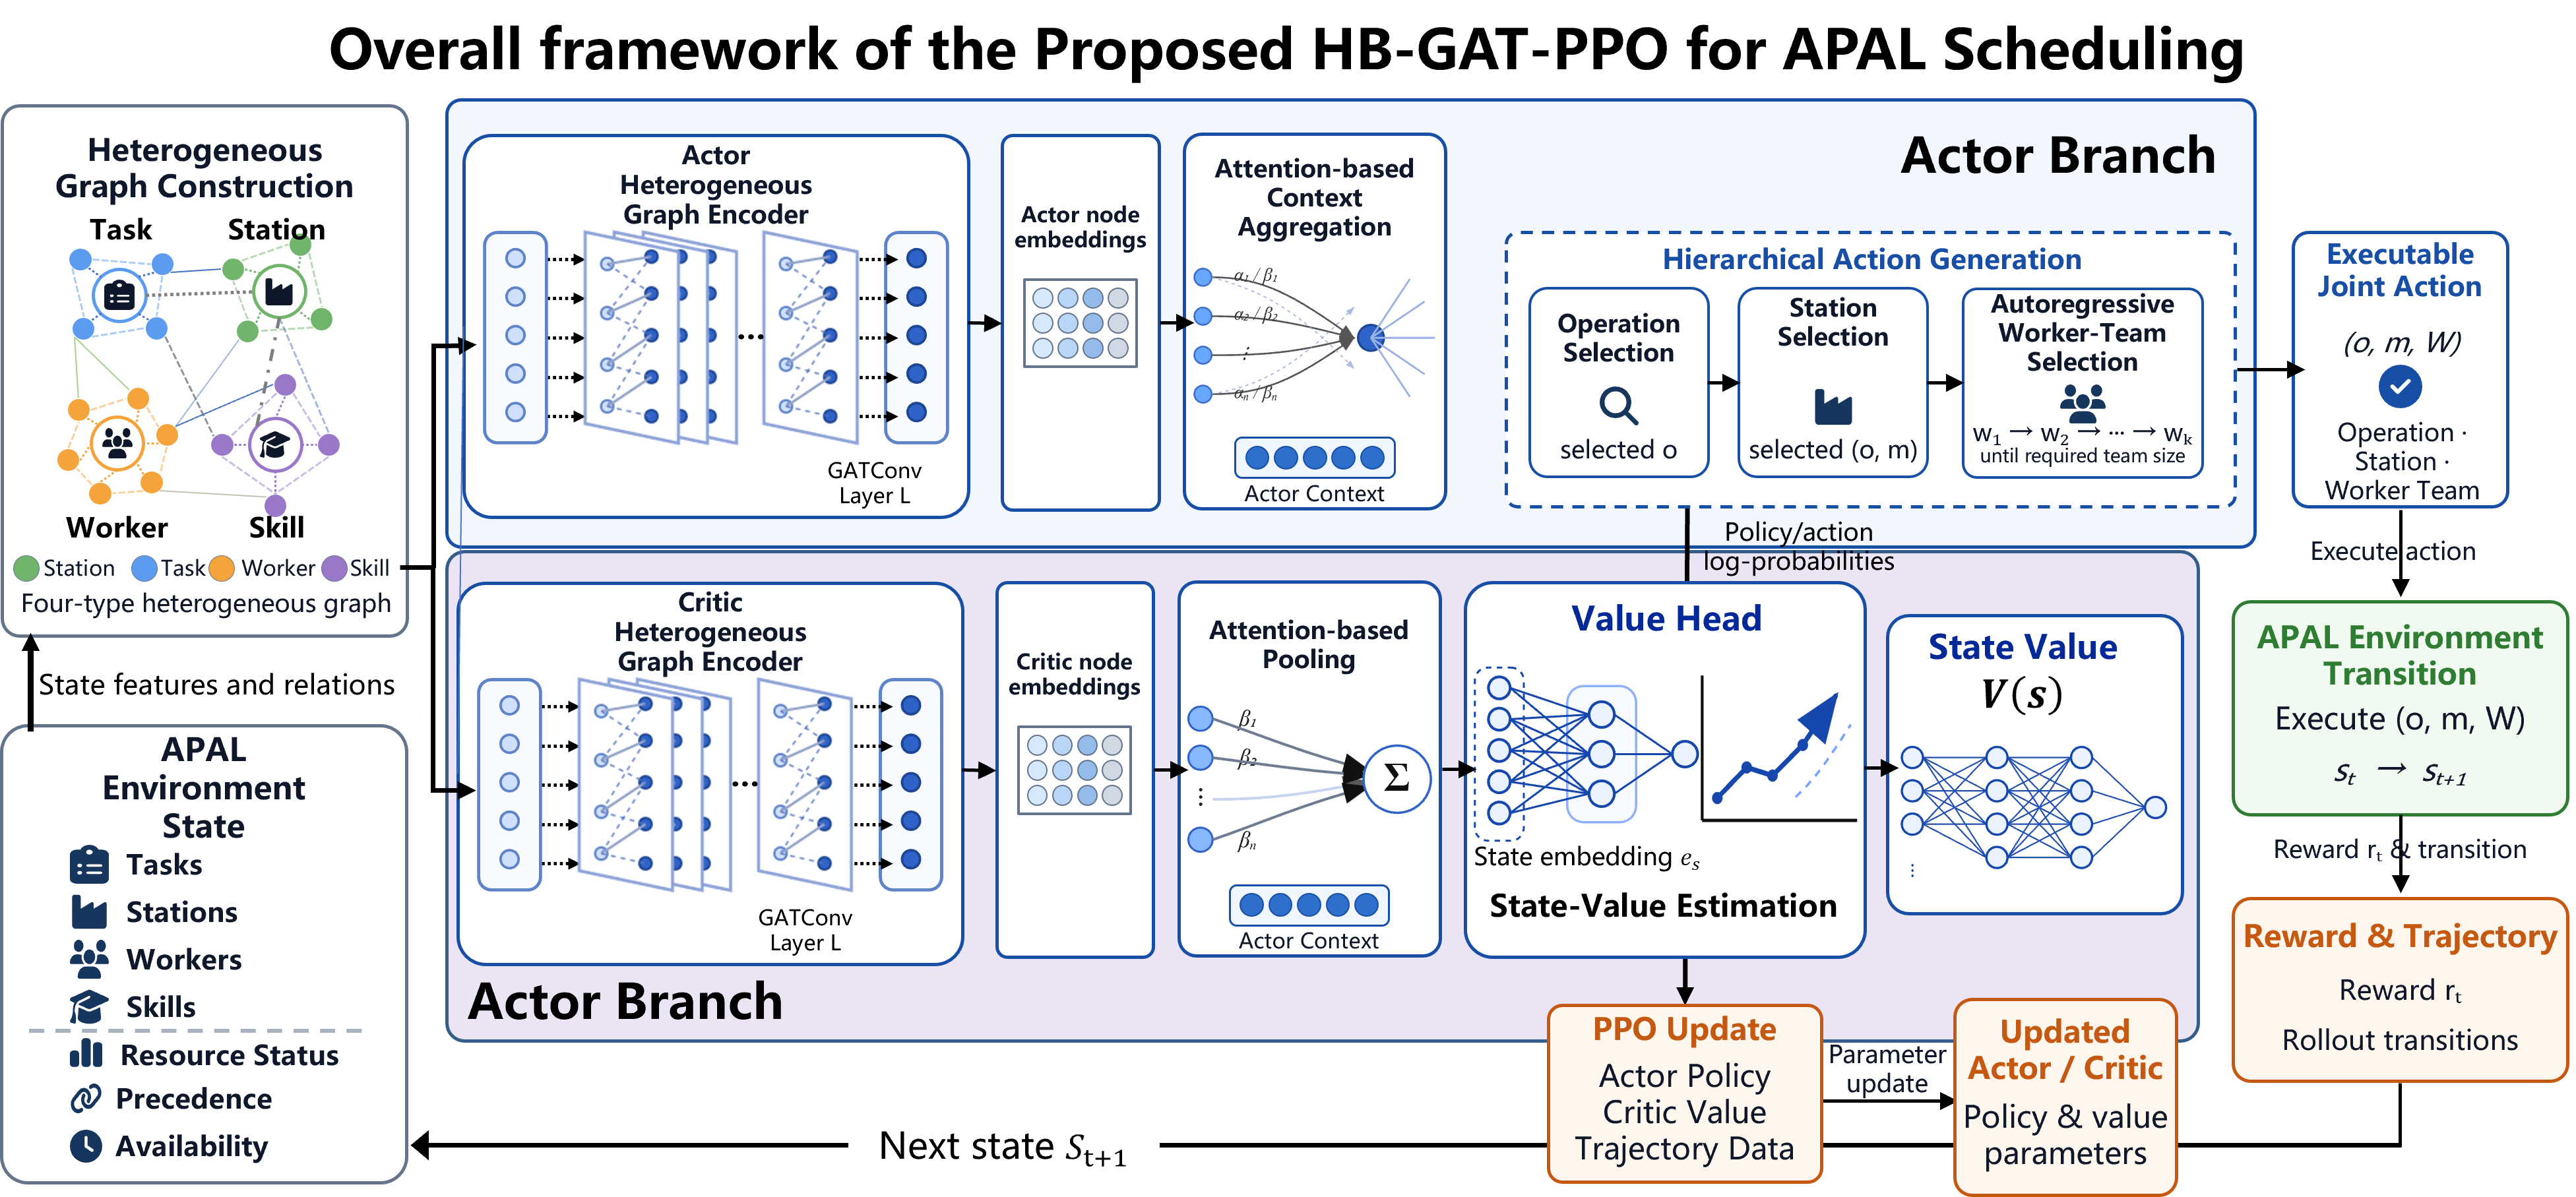
\includegraphics[width=0.92\textwidth,height=0.22\textheight,keepaspectratio]{figures/fig2.png}
\vspace{2pt}
\parbox{\textwidth}{\footnotesize \textbf{图 2　HGP-PPO 总体框架。} APAL 环境状态首先被转换为由 Operation、Station、Worker 和 Skill 构成的四类异构图。Actor 与 Critic 使用相互独立的异构图编码器：Actor 经注意力上下文聚合后依次选择 Operation、Station 和给定人数的 Worker 团队，形成可执行联合动作 $(o,m,W)$；Critic 汇聚图状态并估计状态价值 $V(s)$。环境执行联合动作后产生下一状态、奖励和轨迹，PPO 据此更新策略与价值网络。}
\end{figure*}

\subsection{异构图表示与全局编码}\label{sec:encoder}

\textbf{四类节点与状态特征。} 在决策步 $t$，环境将 APAL 状态构建为异构图 $G_t=(\mathcal{V}_t,\mathcal{E}_t)$，其中节点集合 $\mathcal{V}_t=\mathcal{O}\cup\mathcal{M}\cup\mathcal{W}\cup\mathcal{K}$ 分别表示工序、站位、工人和技能节点。工序节点集合 $\mathcal{O}=\mathcal{O}^{+}\cup\mathcal{O}^{0}$ 包含物理工序与源工艺图中保留的辅助工艺结构节点。结构节点工时为零且无物理资源需求；其保留在图中参与图编码，但排除在可调度动作之外。固定设置 $|\mathcal{K}|=5$。Worker 采用五维多热编码，物理工序采用五维独热编码。四类节点的输入特征见表 II，关系类型见表 III。

\begin{table}[!t]
\centering
\caption{四类节点的输入状态信息（Input State Features）}
\label{tab:node_features}
\setlength{\tabcolsep}{3pt}
\renewcommand{\arraystretch}{1.0}
\begin{adjustbox}{max width=\columnwidth}
\begin{tabular}{@{}lp{6.8cm}@{}}
\toprule
\textbf{节点类型} & \textbf{主要状态特征} \\
\midrule
Operation & 归一化工时 $\widetilde p_i$、调度状态、五维技能需求、团队人数 $q_i$、物料释放时间；重调度追加基准开工、基准站位、团队规模、冻结与延误标记 \\
Station & 累计人时负荷、已绑定与未绑定工人比例、槽位等待时间、可用并发槽位数 \\
Worker & 基础效率 $\eta_w$、五维技能资质、等待时间、空闲标记、站位绑定 $\ell_w$ \\
Skill & 技能类别索引、合格工人工头数、可用容量以及合格工人平均效率 \\
\bottomrule
\end{tabular}
\end{adjustbox}
\vspace{2pt}
\par\noindent{\scriptsize 注：工序特有的资源需求仅适用于物理工序。}\par
\end{table}

连续特征采用实例内生尺度归一化：令 $\bar p = \frac{1}{|\mathcal{O}^{+}|}\sum_{i\in\mathcal{O}^{+}}p_i^{\mathrm{std}}$，工时归一化为 $\widetilde p_i = p_i^{\mathrm{std}}/\bar p$；工人和站位等待量采用对数缩放；站位人时负荷相对于理想均分负荷、全线总负荷及当前最大负荷联合表示；重调度时间偏移相对于基准时域 $T_{\mathrm{ref}}^0$ 归一化。

\textbf{关系类型与动态图更新。} 异构图定义表 III 所列的八类有向关系。工艺前序及技能供需关系在实例内保持静态，而工序---站位和工序---工人关系随联合决策执行动态加入图中。

\begin{table}[!t]
\centering
\caption{异构图关系类型与动态更新（Heterogeneous Graph Relations）}
\label{tab:relations}
\setlength{\tabcolsep}{3pt}
\renewcommand{\arraystretch}{1.0}
\begin{adjustbox}{max width=\columnwidth}
\begin{tabular}{@{}llcl@{}}
\toprule
\textbf{关系名称} & \textbf{源节点 $\to$ 目标节点} & \textbf{更新机制} & \textbf{物理语义} \\
\midrule
precedes & Operation $\to$ Operation & 静态 & 工艺先后序依赖 \\
assigned-to & Operation $\to$ Station & 动态 & 工序站位分配 \\
has-task & Station $\to$ Operation & 动态 & 站位当前所派工序 \\
done-by & Operation $\to$ Worker & 动态 & 工序指定执行团队 \\
has-skill & Worker $\to$ Skill & 回合内固定 & 工人持有技能资质 \\
provided-by & Skill $\to$ Worker & 回合内固定 & 具备该技能的工人 \\
requires & Operation $\to$ Skill & 静态 & 工序所需技能类别 \\
required-by & Skill $\to$ Operation & 静态 & 需要该技能的工序 \\
\bottomrule
\end{tabular}
\end{adjustbox}
\end{table}

\textbf{Skill Hub 与图注意力编码。} 技能节点作为工序需求与人员供给之间的中继枢纽（Skill Hub），使共享技能需求的工序和多技能工人能够通过显式中继参与信息交互。节点原始特征经类型特定映射投影至隐空间 $\mathbf h_v^{(0)}=f_X(\mathbf x_v), v\in\mathcal{V}^X, X\in\{O,M,W,K\}$。采用关系特定的 GATv2 层\cite{brody2022}进行消息传递：
\begin{align}
e_{uv}^{(r,\ell,h)} &= \mathbf a_{r,h}^{(\ell)\top}\operatorname{LeakyReLU}\left(\mathbf W_{s,r,h}^{(\ell)}\mathbf h_u^{(\ell-1)} + \mathbf W_{t,r,h}^{(\ell)}\mathbf h_v^{(\ell-1)}\right), \\
\alpha_{uv}^{(r,\ell,h)} &= \frac{\exp(e_{uv}^{(r,\ell,h)})}{\sum_{z\in\mathcal N_r(v)}\exp(e_{zv}^{(r,\ell,h)})}.
\end{align}
聚合各关系的多头消息后，节点嵌入经残差更新：
\begin{equation}
\mathbf h_v^{(\ell)} = \mathbf h_v^{(\ell-1)} + \operatorname{LeakyReLU}\left(\sum_{r\in\mathcal R_{\mathrm{in}}(v)}\mathbf m_v^{(r,\ell)}\right).
\end{equation}

\textbf{类型级全局注意力池化。} Actor 分别对 Station、Operation 和 Worker 节点执行学习式注意力池化：
\begin{equation}
\beta_v^X = \frac{\exp(a_X(\mathbf h_v))}{\sum_{u\in\mathcal V^X}\exp(a_X(\mathbf h_u))}, \quad \mathbf g_X = \sum_{v\in\mathcal V^X}\beta_v^X\mathbf h_v,
\end{equation}
拼接为全图上下文 $\mathbf g_t = [\mathbf g_M \,\|\, \mathbf g_O \,\|\, \mathbf g_W] \in \mathbb R^{3d}$。Critic 采用独立参数的同构池化层估计状态价值 $V(s_t)$。

\subsection{自回归约束联合解码}\label{sec:decoder}

\textbf{联合动作概率分解。} 为规避对完整团队组合的显式枚举，策略将联合动作分解为工序、条件站位与 $q_{i_t}$ 个条件工人选择步骤。令 $\mathbf w_t=(w_t^{(1)},\dots,w_t^{(q_{i_t})})$ 表示有序工人序列，$W_t$ 为对应无序团队集合：
\begin{equation}
\begin{aligned}
\pi_\theta(\widetilde a_t\mid s_t) ={}& \pi_O(i_t\mid s_t)\,\pi_M(m_t\mid s_t,i_t) \\
&\times \prod_{r=1}^{q_{i_t}}\pi_W\left(w_t^{(r)}\mid s_t,i_t,m_t,\mathbf w_t^{(<r)}\right).
\end{aligned}
\end{equation}
PPO 采用有序轨迹 $\widetilde a_t$ 计算联合对数似然，物理环境执行采用无序集合 $W_t$。

\textbf{工序与站位指针。} 工序指针结合全局上下文 $\mathbf g_t$ 与工序嵌入 $\mathbf h_i$ 打分；站位指针以所选工序 $\mathbf h_{i_t}$ 为条件对五个物理站位打分：
\begin{align}
u_{i,t}^O &= \mathbf a_O^{\top}\tanh(\mathbf W_g\mathbf g_t + \mathbf W_O\mathbf h_i), \\
\pi_O(i\mid s_t) &= \exp(u_{i,t}^O)\Big/\textstyle\sum_{j\in\mathcal F_t^O}\exp(u_{j,t}^O), \\
u_{m,t}^M &= \mathbf a_M^{\top}\tanh(\mathbf W_{OM}\mathbf h_{i_t} + \mathbf W_M\mathbf h_m), \\
\pi_M(m\mid s_t,i_t) &= \exp(u_{m,t}^M)\Big/\textstyle\sum_{n\in\mathcal F_{i_t,t}^M}\exp(u_{n,t}^M).
\end{align}

\textbf{定长团队构造与 Worker Pointer。} 选定工序与站位后，Worker Pointer 在子步 $r\in\{1,\dots,q_{i_t}\}$ 中结合查询 $\mathbf q_t^{(r)}$ 与候选键 $\mathbf k_{w,t}^{(r)}$ 打分：
\begin{align}
u_{w,t}^{(r)} &= \mathbf v_W^{\top}\tanh\left(\mathbf q_t^{(r)} + \mathbf k_{w,t}^{(r)}\right), \\
\pi_W(w\mid s_t,i_t,m_t,\mathbf w_t^{(<r)}) &= \exp(u_{w,t}^{(r)})\Big/\textstyle\sum_{v\in\mathcal F_{W,t}^{(r)}}\exp(u_{v,t}^{(r)}).
\end{align}
非法候选得分置为 $-\infty$。查询 $\mathbf q_t^{(r)}$ 与键 $\mathbf k_{w,t}^{(r)}$ 融合了技能压力、动态 EFT 及边际稀缺度（详见附录 A）。

\textit{内生工人---站位绑定（Endogenous worker--station binding）：}
当初始未分配站位的工人被指派给站位 $m_t$ 的工序时，该工人在此排程周期的剩余阶段内专用归属于该站位。所得站位归属在后续重调度中严格继承：
\begin{equation}
\ell_{w,t+1} = \begin{cases} m_t, & \ell_{w,t}=\varnothing \ \text{且}\ w\in W_t, \\ \ell_{w,t}, & \text{其他情况}. \end{cases}
\end{equation}

\subsection{PPO 学习与迁移}\label{sec:learning}

令连续性标记 $b_t=(1-d_t)(1-u_t)$，时序差分误差 $\delta_t$ 与广义优势估计（GAE）\cite{schulman2016}为：
\begin{equation}
\delta_t = r_t + \gamma b_t V_{\phi^-}(s_{t+1}) - V_{\phi^-}(s_t), \quad \widehat A_t = \delta_t + \gamma\lambda b_t \widehat A_{t+1}.
\end{equation}
裁剪 PPO 损失\cite{schulman2017}与总优化目标为：
\begin{equation}
\begin{aligned}
\mathcal L_{\mathrm{policy}}(\theta) = -\mathbb E_t\Big[ \min\Big( &r_t^{\mathrm{PPO}}(\theta)\widetilde A_t, \\
&\operatorname{clip}(r_t^{\mathrm{PPO}}(\theta), 1-\epsilon, 1+\epsilon)\widetilde A_t \Big) \Big],
\end{aligned}
\end{equation}
\begin{equation}
\mathcal L = \mathcal L_{\mathrm{policy}}(\theta) + c_V \mathbb E_t[(V_\phi(s_t)-R_t)^2] - c_H \overline H.
\end{equation}
异构图编码器与指针解码器采用共享参数与动态掩码，解耦了特定规模工序与工人数的绑定。在重调度阶段，工序节点特征维度由 18 维扩充至 24 维，第一层工序输入映射矩阵相应展宽。图编码器、池化层与指针解码器等兼容参数直接继承自初始排程模型；工序投影层中对应原特征维度的参数完全继承，新增维度随机初始化。随后策略网络在继承既有工人站位绑定的基础上，面向扰动环境与综合稳定性目标 $S(\pi^r)$ 继续微调训练，实现有效知识迁移。

\section{实验与结果}\label{sec:experiments}

\subsection{评价问题与实验协议}\label{sec:exp_protocol}

实验围绕五个核心评价问题（EQs）展开：
\begin{itemize}
\item \textbf{EQ1（跨规模外推）}：同一锁定策略在无需微调的条件下，能否直接求解 283 至 3182 道物理工序的真实工厂实例？
\item \textbf{EQ2（联合解码质量）}：工序---站位---具体工人团队的自回归指针解码在周期跨度 $H=C_{\max}$ 上是否优于传统派工规则、启发式搜索与基线模型？
\item \textbf{EQ3（关键结构消融）}：异构图注意力编码、工人---站位内生绑定机制以及完整三层联合决策是否对应 APAL 的实际物理约束？
\item \textbf{EQ4（在线时间扩展）}：神经前向推断与传统逐实例搜索在不同工序规模下的端到端重调度耗时表现如何？
\item \textbf{EQ5（延误重调度恢复）}：所提架构在物料就绪延误下，能否兼顾排程物理合法性、完工节拍与基准方案的计划稳定性？
\end{itemize}

\textit{数据集划分：}
实验严格使用训练集、验证集与测试集：
\begin{itemize}
\item \textit{训练集（Training set）：} 24 个合成变体，包含 400--800 道物理工序，用于模型参数梯度更新；
\item \textit{验证集（Validation set）：} 6 个实例与 54 个延误场景，用于超参数选择、早停与检查点挑选；
\item \textit{测试集（Test set）：} 4 个真实工厂实例（表 IV）与 36 个固定扰动场景，保留用于模型选择后的最终评估，不进行进一步调优。
\end{itemize}

\textbf{硬性合法性门槛。} 排程必须 100\% 满足工艺前序、站位单调性、5 个物理站位容量、给定团队人数 $q_i$、技能匹配、工人时间互斥及工人---站位锁定约束；重调度还必须满足计划冻结边界 $\tau^r$ 继承、物料到货延误与既有工人绑定继承。所有方案必须通过独立排程校验器审计，完整率（$R_{\mathrm{complete}}=1$）与合法率（$R_{\mathrm{valid}}=1$）作为进入质量排序的硬性前置门槛。

\subsection{评价实例、基线与统计口径}\label{sec:instances}

测试集包含源自真实工厂 APAL 工艺数据的四个实例：Medium（283 道物理工序）、Large（680）、Industrial-I（2,338）与 Industrial-II（3,182）。所有四个实例均包含 5 个物理站位。

\begin{table}[!t]
\centering
\caption{真实工厂 APAL 测试实例（Real Factory APAL Test Instances）}
\label{tab:instances}
\setlength{\tabcolsep}{8pt}
\renewcommand{\arraystretch}{1.02}
\begin{adjustbox}{max width=\columnwidth}
\begin{tabular}{@{}lccc@{}}
\toprule
\textbf{实例名称} & \textbf{物理工序数} & \textbf{站位数} & \textbf{实验角色} \\
\midrule
Medium & 283 & 5 & Test \\
Large & 680 & 5 & Test \\
Industrial-I & 2,338 & 5 & Test \\
Industrial-II & 3,182 & 5 & Test \\
\bottomrule
\end{tabular}
\end{adjustbox}
\vspace{2pt}
\par\noindent{\scriptsize 注：实例规模仅统计物理工序数。Medium、Large、Industrial-I 与 Industrial-II 的源工艺图中分别额外包含 7、35、64 和 117 个工艺结构节点（总工艺节点数对应为 290、715、2,402 和 3,299）。}\par
\end{table}

\begin{table}[!t]
\centering
\caption{比较方法、决策依据与搜索预算（Comparison Methods）}
\label{tab:baselines}
\setlength{\tabcolsep}{3pt}
\renewcommand{\arraystretch}{0.98}
\begin{adjustbox}{max width=\columnwidth}
\begin{tabular}{@{}lll@{}}
\toprule
\textbf{类别} & \textbf{方法} & \textbf{决策依据／搜索预算} \\
\midrule
派工规则 & SPT\cite{smith1956} / LPT & 按标准工时最短／最长优先选择工序 \\
派工规则 & ES / CPM\cite{kelley1961} / MSL & 按最早开始／关键路径／最小松弛优先 \\
派工规则 & Random & 固定随机种子下的随机优先权 \\
元启发式 & Beam Search\cite{ow1988} & 优先级搜索；初始：$w=4, b=4$；重调度：$w=2, b=2$ \\
元启发式 & IG\cite{ruiz2007} & 破坏---重构；初始：160代；重调度：3代 \\
元启发式 & SA\cite{kirkpatrick1983} & 模拟退火；初始：120代；重调度：3代 \\
RL 基线 & L2D-PPO-APAL & 适配 APAL 的学习式图派工策略 \\
RL 基线 & Graph-DDQN-APAL & 适配 APAL 的图值函数强化学习 \\
参考组 & NoReschedule & 负控制组：保留基准方案，不主动修复 \\
启发式修复 & StabilityAware / CPM & 兼顾开工扰动与关键路径的复合规则 \\
\bottomrule
\end{tabular}
\end{adjustbox}
\end{table}

\textbf{评价指标与统计推断。} 初始排程以周期跨度 $H=C_{\max}$（式\eqref{eq:cmax}）为主要指标，采用确定性 masked argmax 作为主比较。重调度在严格满足合法性前提下，以加权综合目标 $S$（式\eqref{eq:reschedule_obj}）为核心指标，并在 36 个配对扰动场景上展开。采用场景配对 Friedman 检验评估 19 种合法方法的全局排序差异，通过双侧 Wilcoxon 符号秩检验（Holm--Bonferroni 校正控制族错误率）与 10,000 次分层 Bootstrap 估计 95\% 置信区间。

\subsection{初始排程主结果与跨规模表现}\label{sec:init_results}

表 VI 汇总了各方法在四个真实工厂 APAL 实例上的确定性解码结果。进入该表的结果均形成完整排程并通过统一合法性校验。本文方法使用同一锁定策略直接处理 Medium 至 Industrial-II 实例，测试期间不更新梯度，也不进行实例特定调参。

\begin{table*}[!t]
\centering
\caption{比较方法与人员预配置消融在四个 APAL 实例上的初始排程 makespan（h，越小越好）}
\label{tab:initial_results}
\setlength{\tabcolsep}{5pt}
\renewcommand{\arraystretch}{1.0}
\begin{adjustbox}{max width=\textwidth}
\begin{tabular}{@{}llrrrrr@{}}
\toprule
\textbf{算法类别} & \textbf{算法名称} & \textbf{Medium} & \textbf{Large} & \textbf{Industrial-I} & \textbf{Industrial-II} & \textbf{四规模等权平均} \\
\midrule
图强化学习 & 本文方法 (Proposed HGP-PPO) & 286.96 & \textbf{489.00} & 1209.96 & \textbf{1623.69} & \textbf{902.40} \\
人员配置消融 & Worker--Station 预配置 & 320.31 & 959.63 & 1605.13 & 2645.84 & 1382.73 \\
学习型基线 & L2D-PPO-APAL & 288.97 & 518.65 & \textbf{1079.44} & 1804.71 & 922.94 \\
学习型基线 & Graph-DDQN-APAL & \textbf{286.77} & 612.29 & 1263.66 & 2049.70 & 1053.11 \\
搜索与元启发式 & IG & 339.05 & 961.10 & 1797.57 & 2759.01 & 1464.18 \\
搜索与元启发式 & Beam Search & 333.43 & 984.30 & 1904.88 & 3272.54 & 1623.79 \\
搜索与元启发式 & SA & 311.78 & 1238.00 & 2417.03 & 3256.29 & 1805.77 \\
优先规则 & LPT & 292.63 & 637.56 & 1497.35 & 2039.50 & 1116.76 \\
优先规则 & Random & 310.62 & 872.52 & 1414.20 & 2170.15 & 1191.87 \\
优先规则 & SPT & 411.57 & 1702.77 & 2479.07 & 3346.37 & 1984.94 \\
优先规则 & MSL & 412.56 & 1608.50 & 2496.05 & 3455.45 & 1993.14 \\
优先规则 & ES-priority & 435.13 & 1773.41 & 2780.24 & 3729.75 & 2179.63 \\
优先规则 & CPM & 387.28 & 1597.92 & 2522.96 & 3430.06 & 1984.55 \\
\bottomrule
\end{tabular}
\end{adjustbox}
\end{table*}

从四规模等权平均结果看，本文方法取得最低的平均 makespan 902.40 h，较 L2D-PPO-APAL 的 922.94 h 降低 2.22\%，Graph-DDQN-APAL 的平均值则为 1053.11 h。图 3(a) 直观给出了各方法在对数坐标下的完工周期跨度扩展趋势。逐实例结果显示，这一优势并非来自所有规模上的一致领先：Graph-DDQN-APAL 在 Medium 实例上以 286.77 h 略低于本文方法的 286.96 h，L2D-PPO-APAL 在 Industrial-I 实例上以 1079.44 h 优于本文方法的 1209.96 h。本文方法在 Large 和 Industrial-II 实例上分别取得 489.00 h 和 1623.69 h 的最低值；其中，在最大的 Industrial-II 实例上，其 makespan 较 L2D-PPO-APAL 缩短 181.02 h，即降低 10.03\%。

规则与逐实例搜索方法表现出更明显的规模退化。规则方法中，LPT 的四规模平均 makespan 最低，为 1116.76 h；搜索与元启发式方法中，IG 的平均值最低，为 1464.18 h。Beam Search 和 SA 的平均 makespan 分别为 1623.79 h 和 1805.77 h。

固定随机解码设置提供了补充的输出稳健性信息。本文方法在四个实例上的随机解码均值依次为 $274.97\pm3.77$、$517.50\pm12.89$、$1070.71\pm101.12$ 和 $1678.47\pm55.94$ h，四规模等权平均为 885.41 h。随机采样在 Medium 和 Industrial-I 上获得更短均值，但在 Large 和 Industrial-II 上较高，说明随机采样并未形成跨规模一致的改进。因此本文仍以确定性解码作为主比较口径。

\subsection{决策架构与网络配置对比及可行性边界}\label{sec:ablations}

为区分人员配置方式、图表示与联合决策层级的作用，表 VII 比较了本文方法及三个结构配置变体。所有方法共享相同的环境约束与合法性评价口径。

\begin{table*}[!t]
\centering
\caption{决策架构与网络配置对比的初始排程结果及重调度合法率}
\label{tab:ablations}
\setlength{\tabcolsep}{5pt}
\renewcommand{\arraystretch}{1.0}
\begin{adjustbox}{max width=\textwidth}
\begin{tabular}{@{}llrrrrrcc@{}}
\toprule
\textbf{模型变体} & \textbf{主要修改点} & \textbf{Medium} & \textbf{Large} & \textbf{Industrial-I} & \textbf{Industrial-II} & \textbf{四规模平均} & \textbf{初始合法数} & \textbf{重调度合法率} \\
\midrule
本文方法 (Full HGP-PPO) & 完整模型（异构图+指针+内生绑定） & 286.96 & 489.00 & 1209.96 & 1623.69 & \textbf{902.40} & 4/4 & 100\% \\
同构 GraphSAGE & 以同构图编码替代异构图编码 & 292.02 & 594.04 & 1323.22 & 1941.29 & 1037.64 & 4/4 & 100\% \\
工序---Station 联合决策 & 不显式选择工人，由规则凑人 & \textbf{267.40} & 565.26 & \textbf{1154.20} & 2073.34 & 1015.05 & 4/4 & 0\% \\
仅工序决策 & Station 与工人由启发式补全 & 269.66 & 779.13 & 不可行 & 不可行 & --- & 2/4 & 100\% \\
\bottomrule
\end{tabular}
\end{adjustbox}
\vspace{2pt}
\par\noindent{\scriptsize 注：初始排程列为确定性解码的 makespan（h，越小越好）；仅在四个实例均合法时计算平均值。重调度合法率按四个规模共 36 个扰动场景统计。}\par
\end{table*}

\begin{figure}[!t]
\centering
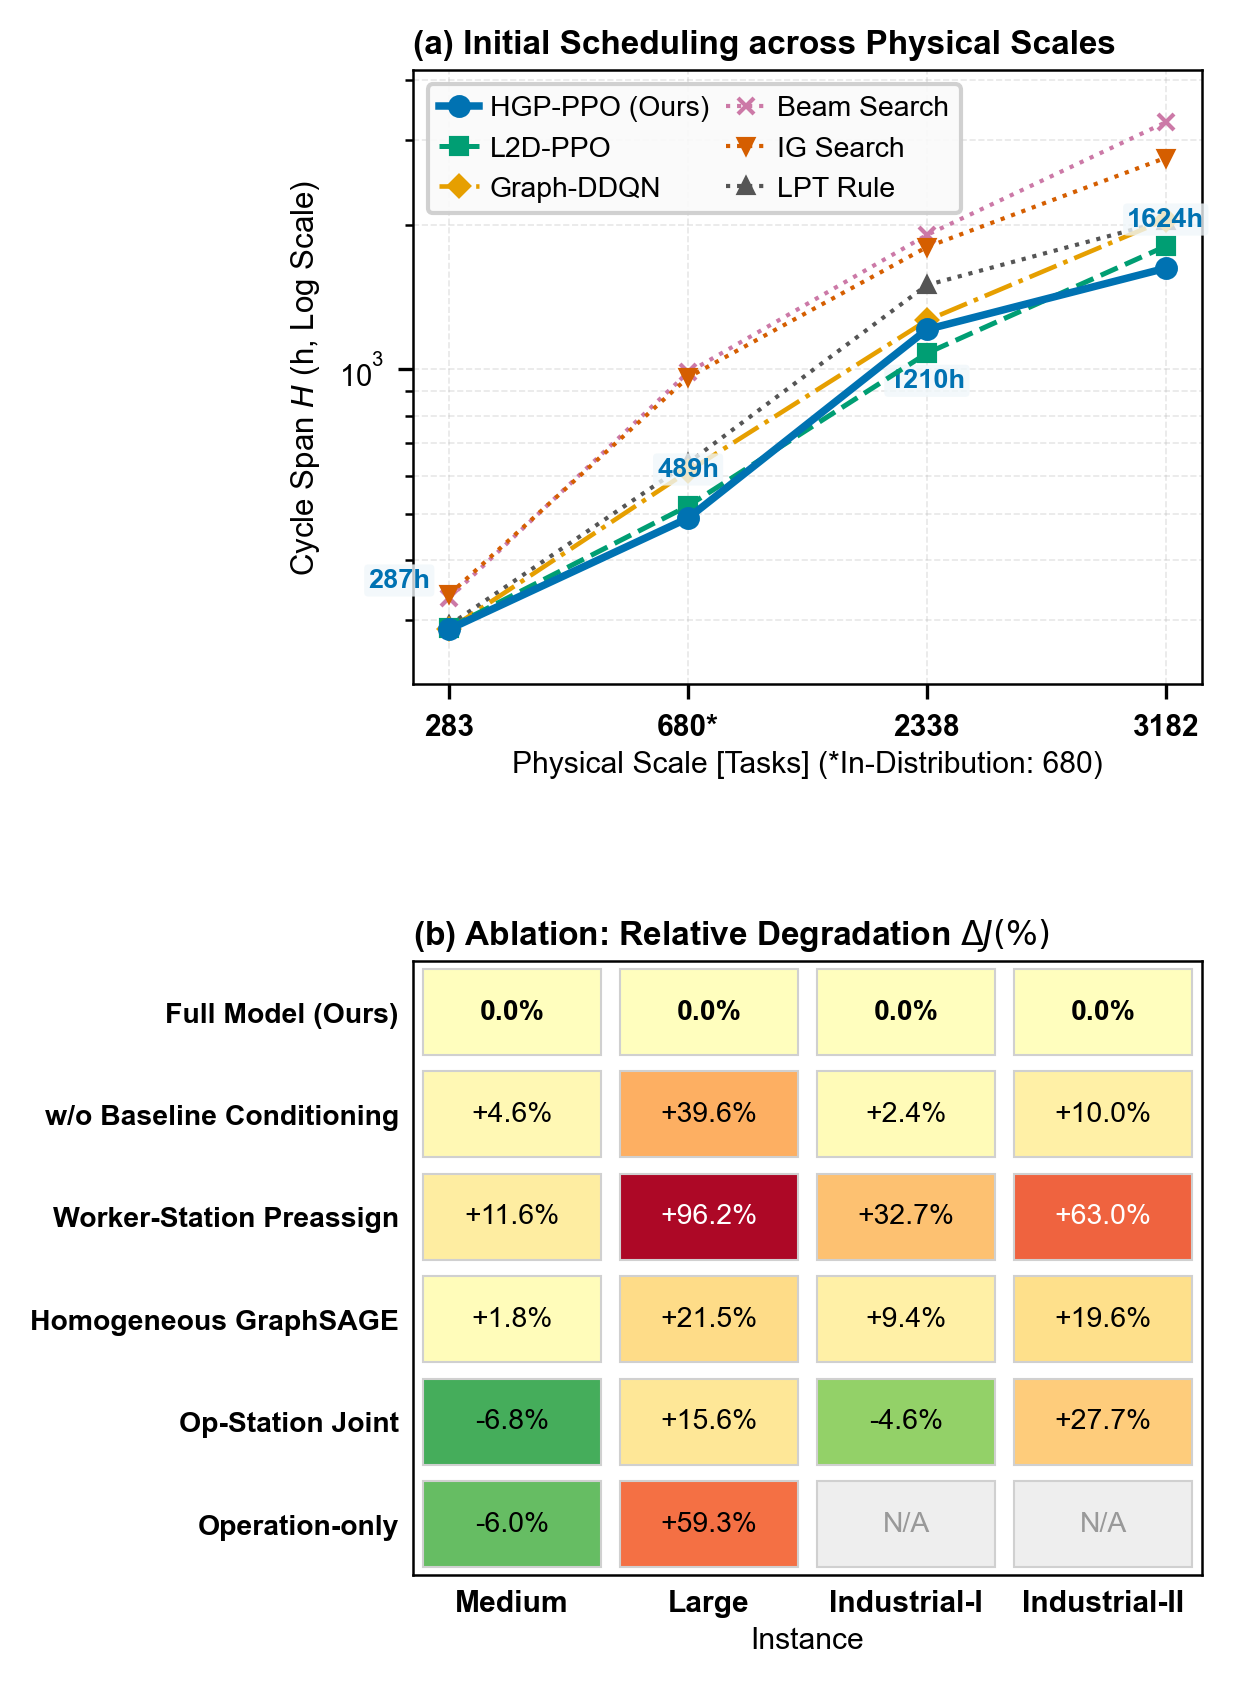
\includegraphics[width=\columnwidth,keepaspectratio]{figures/fig3_initial_and_ablation.png}
\vspace{2pt}
\parbox{\columnwidth}{\footnotesize \textbf{图 3　跨物理规模初始排程完工周期与决策架构消融对比。} (a) 6 种代表性方法在 283、680、2338 和 3182 尺度上的完工周期跨度 $H$（对数坐标，实线标出本文方法）；(b) 决策架构变体相对于完整模型（Full Model）在 Medium、Large、Industrial-I 与 Industrial-II 上的工期相对劣化率 $\Delta J(\%)$ 矩阵。}
\end{figure}

Worker--Station 预配置消融在排程开始前固定工人的 Station 归属，策略只能在既定归属内选择具体成员。该变体在四个规模上均能生成合法排程，但确定性解码的平均 makespan 为 1382.73 h，较本文方法的 902.40 h 高 53.2\%。该结果表明，排程前预先固定工人站位归属严重限制了人力资源自适应匹配各站位动态负荷的能力。

结合图 3(b) 的消融矩阵，同构 GraphSAGE 在四个规模上均能生成合法排程，但平均 makespan 由 902.40 h 增至 1037.64 h（劣化 +15.0\%），说明区分工序、Station、工人与技能关系有助于维持跨规模解质量。工序---Station 变体在部分规模上取得更短工期，却在重调度中无法完成全部待排工序（0\% 重调度合法率）；仅工序变体则在两个较大初始排程实例上不可行。由此可见，较浅决策在小规模实例上的局部优势不能替代跨规模可行性检验。

\subsection{物料延误下的重调度结果}\label{sec:resched_results}

表 VIII 比较了各方法在四个规模、三种延误强度和三个触发阶段组成的 36 个配对场景上的重调度结果。表中完整列出进入 Friedman 统计的 19 种合法方法，并保留 No\allowbreak{}Reschedule 作为负控制；重调度合法率为 0\% 的工序---Station 变体不进入质量统计。综合分 $S$ 越小越好。

\begin{table*}[!t]
\centering
\caption{物料延误重调度的综合分与平均 makespan（36 场景）}
\label{tab:reschedule_results}
\setlength{\tabcolsep}{3pt}
\renewcommand{\arraystretch}{0.98}
\begin{adjustbox}{max width=\textwidth}
\begin{tabular}{@{}llccccccc@{}}
\toprule
\textbf{算法类别} & \textbf{算法名称} & \textbf{Medium} & \textbf{Large} & \textbf{Industrial-I} & \textbf{Industrial-II} & \textbf{平均 $S$} & \textbf{平均 makespan（h）} & \textbf{合法率} \\
\midrule
图强化学习 & 本文方法 (Proposed HGP-PPO) & 0.9572 / 297.7 & 0.7621 / 674.9 & 0.8627 / 1223.9 & 0.8224 / 1709.5 & \textbf{0.8511} & 976.5 & 100\% \\
模型变体 & 不含基准归属条件特征的前代模型 & 0.9700 / 300.1 & 0.8242 / 682.5 & 0.9186 / 1239.2 & 1.0588 / 1786.6 & 0.9429 & 1002.1 & 100\% \\
结构对比 & 同构 GraphSAGE & 1.2236 / 318.9 & 1.0447 / 682.4 & 1.0310 / 1263.2 & 1.1599 / 1806.8 & 1.1148 & 1017.8 & 100\% \\
结构对比 & 仅工序决策 & 0.9592 / 296.9 & 1.2479 / 678.6 & 1.0825 / 1223.8 & 1.6577 / 1903.3 & 1.2368 & 1025.7 & 100\% \\
学习型基线 & L2D-PPO-APAL & 0.9439 / 301.3 & 0.8441 / 663.3 & 0.8401 / 1223.9 & 1.0325 / 1764.9 & 0.9152 & 988.3 & 100\% \\
学习型基线 & Graph-DDQN-APAL & 1.0414 / 306.6 & 1.0714 / 672.8 & 0.9394 / 1223.9 & 0.8716 / 1709.9 & 0.9810 & 978.3 & 100\% \\
元启发式搜索 & Beam\allowbreak{}Search\allowbreak{}Repair & 1.0575 / 322.9 & 1.0763 / 752.4 & 1.2596 / 1403.6 & 1.3626 / 1987.2 & 1.1890 & 1116.5 & 100\% \\
元启发式搜索 & Iterated\allowbreak{}Greedy\allowbreak{}Repair & 1.0312 / 319.1 & 1.6770 / 783.1 & 1.6892 / 1454.1 & 1.3655 / 1987.5 & 1.4407 & 1135.9 & 100\% \\
元启发式搜索 & Simulated\allowbreak{}Annealing\allowbreak{}Repair & 1.1431 / 323.6 & 2.2088 / 814.1 & 1.8923 / 1484.4 & 1.4394 / 2001.8 & 1.6709 & 1156.0 & 100\% \\
启发式修复 & Hybrid\allowbreak{}CPM\allowbreak{}Stability\allowbreak{}Repair & 1.1337 / 294.2 & 1.0463 / 675.4 & 0.9952 / 1223.9 & 0.7560 / 1665.9 & 0.9828 & \textbf{964.9} & 100\% \\
启发式修复 & Stability\allowbreak{}Aware\allowbreak{}Repair & 0.9913 / 310.4 & 0.7554 / 682.7 & 0.8045 / 1229.4 & 0.9591 / 1752.8 & 0.8776 & 993.8 & 100\% \\
启发式修复 & Takt\allowbreak{}Aware\allowbreak{}Repair & 0.9103 / 323.8 & 1.0759 / 775.7 & 1.0398 / 1307.4 & 0.9073 / 1816.4 & 0.9833 & 1055.8 & 100\% \\
启发式修复 & Release\allowbreak{}Aware\allowbreak{}Repair & 0.7844 / 316.8 & 1.4584 / 770.5 & 1.1644 / 1369.4 & 1.1556 / 1901.5 & 1.1407 & 1089.5 & 100\% \\
启发式修复 & Bottleneck\allowbreak{}Skill\allowbreak{}Repair & 0.9667 / 326.4 & 1.4732 / 768.0 & 1.4282 / 1404.7 & 0.8398 / 1827.5 & 1.1770 & 1081.7 & 100\% \\
启发式修复 & SPTRepair & 1.0188 / 333.3 & 0.9794 / 758.4 & 1.1850 / 1373.5 & 1.2038 / 1914.2 & 1.0967 & 1094.9 & 100\% \\
启发式修复 & Full\allowbreak{}Reschedule\allowbreak{}CPM & 1.3579 / 332.0 & 1.5415 / 778.9 & 1.5528 / 1384.3 & 1.1864 / 1875.6 & 1.4097 & 1092.7 & 100\% \\
启发式修复 & CPMRepair & 1.3513 / 331.1 & 1.5147 / 773.9 & 1.5968 / 1396.1 & 1.1838 / 1880.2 & 1.4116 & 1095.3 & 100\% \\
启发式修复 & LPTRepair & 1.5492 / 345.0 & 2.6828 / 836.3 & 1.9494 / 1456.0 & 1.3546 / 1922.1 & 1.8840 & 1139.9 & 100\% \\
启发式修复 & Random\allowbreak{}Repair & 1.5427 / 351.7 & 3.2131 / 943.2 & 2.6982 / 1673.2 & 1.9854 / 2153.4 & 2.3599 & 1280.4 & 100\% \\
负控制组 & No\allowbreak{}Reschedule & --- & --- & --- & --- & 不适用 & 不适用 & 0\% \\
\bottomrule
\end{tabular}
\end{adjustbox}
\vspace{2pt}
\par\noindent{\scriptsize 注：四个规模列均为``$S$ / makespan（h）''。$S$ 先在每个场景中按基准排程时域 $T_{\mathrm{ref}}^0$ 归一化，再进行实例内和跨实例等权平均。}\par
\end{table*}

本文方法在 36 个场景中保持 100\% 合法，并取得最低的跨规模平均综合分 0.8511。其综合分中位数和 IQM 分别为 0.7415 和 0.7670，均低于 Stability\allowbreak{}Aware\allowbreak{}Repair（0.7574 和 0.7878）及 L2D-PPO-APAL（0.7592 和 0.8042）。本文方法的 ARD 为 26.60\%，在 19 种合法方法中最低；其综合分观测范围为 1.0089，同样为所有合法方法中的最小值。Friedman 检验表明 19 种合法方法的总体排序存在差异（$\chi_F^2(18)=369.20$，$p<0.001$），本文方法的平均秩最低，为 4.56，L2D-PPO-APAL 和 Stability\allowbreak{}Aware\allowbreak{}Repair 分别为 4.86 和 5.00。

表 IX 进一步拆分代表性方法的物理分项。

\begin{table}[!t]
\centering
\caption{代表性方法的重调度原始物理分项分解}
\label{tab:raw_components}
\setlength{\tabcolsep}{2.5pt}
\renewcommand{\arraystretch}{0.92}
\begin{adjustbox}{max width=\columnwidth}
\begin{tabular}{@{}lrrrrrr@{}}
\toprule
\textbf{方法名称} & $C_{\max}$ (h) & $\Delta_{\mathrm{ref}}$ (h) & $\bar D_{\mathrm{start}}$ (h) & $R_{\mathrm{sta}}$ (\%) & $R_{\mathrm{team}}$ (\%) & $S$ \\
\midrule
本文方法 (HGP-PPO) & 976.49 & 29.51 & \textbf{30.85} & 2.12 & 95.60 & \textbf{0.8511} \\
L2D-PPO-APAL & 988.33 & 42.11 & 45.54 & 1.93 & 95.87 & 0.9152 \\
Graph-DDQN-APAL & 978.32 & 29.63 & 56.31 & 2.02 & 96.05 & 0.9810 \\
BeamSearchRepair & 1116.52 & 167.19 & 108.85 & 0.54 & 0.70 & 1.1890 \\
HybridCPMStability & \textbf{964.87} & \textbf{18.79} & 61.76 & 1.85 & 93.53 & 0.9828 \\
StabilityAwareRepair & 993.85 & 45.22 & 33.88 & 1.73 & 94.76 & 0.8776 \\
\bottomrule
\end{tabular}
\end{adjustbox}
\vspace{2pt}
\par\noindent{\scriptsize 注：$R_{\mathrm{team}}$ 按可重排工序的无序团队进行二值判定：任一成员改变即计为变更，不代表跨 Station 调动。}\par
\end{table}

相对 Stability\allowbreak{}Aware\allowbreak{}Repair，本文方法的平均 makespan 缩短 17.36 h，且在 32 个场景中较短、4 个场景中较长；基准超限量平均减少 15.71 h，对应 29 胜、3 平和 4 负。两项分项差异在 Holm 校正后均保持显著（$p<0.001$）。相对 L2D-PPO-APAL，本文方法的平均 makespan、基准超限量和开工时间偏差分别减少 11.84 h、12.60 h 和 14.70 h（开工偏差均值降低 32.3\%）。

\begin{table*}[!t]
\centering
\caption{本文方法与两个最近基线的重调度配对统计（Paired Statistics）}
\label{tab:paired_stats}
\setlength{\tabcolsep}{4pt}
\renewcommand{\arraystretch}{0.95}
\begin{adjustbox}{max width=\textwidth}
\begin{tabular}{@{}lcccccc@{}}
\toprule
\textbf{对照基线} & \textbf{平均 $S$ 差值（本文−对照）} & \textbf{相对降低率} & \textbf{胜／平／负（W / T / L）} & $p_{\mathrm{Holm}}$ & $r_{\mathrm{rb}}$ & \textbf{分层 Bootstrap 95\% CI} \\
\midrule
L2D-PPO-APAL & −0.0640 & 7.00\% & 19／0／17 & 0.7237 & −0.069 & [−0.1344, −0.0023] \\
StabilityAwareRepair & −0.0265 & 3.01\% & 22／0／14 & 0.5498 & −0.210 & [−0.0652, 0.0110] \\
\bottomrule
\end{tabular}
\end{adjustbox}
\vspace{2pt}
\par\noindent{\scriptsize 注：负差值表示本文方法具有较低综合分。$p_{\mathrm{Holm}}$ 为校正后的双侧 Wilcoxon 结果。Bootstrap 区间基于 10,000 次重采样。}\par
\end{table*}

\begin{figure*}[!t]
\centering
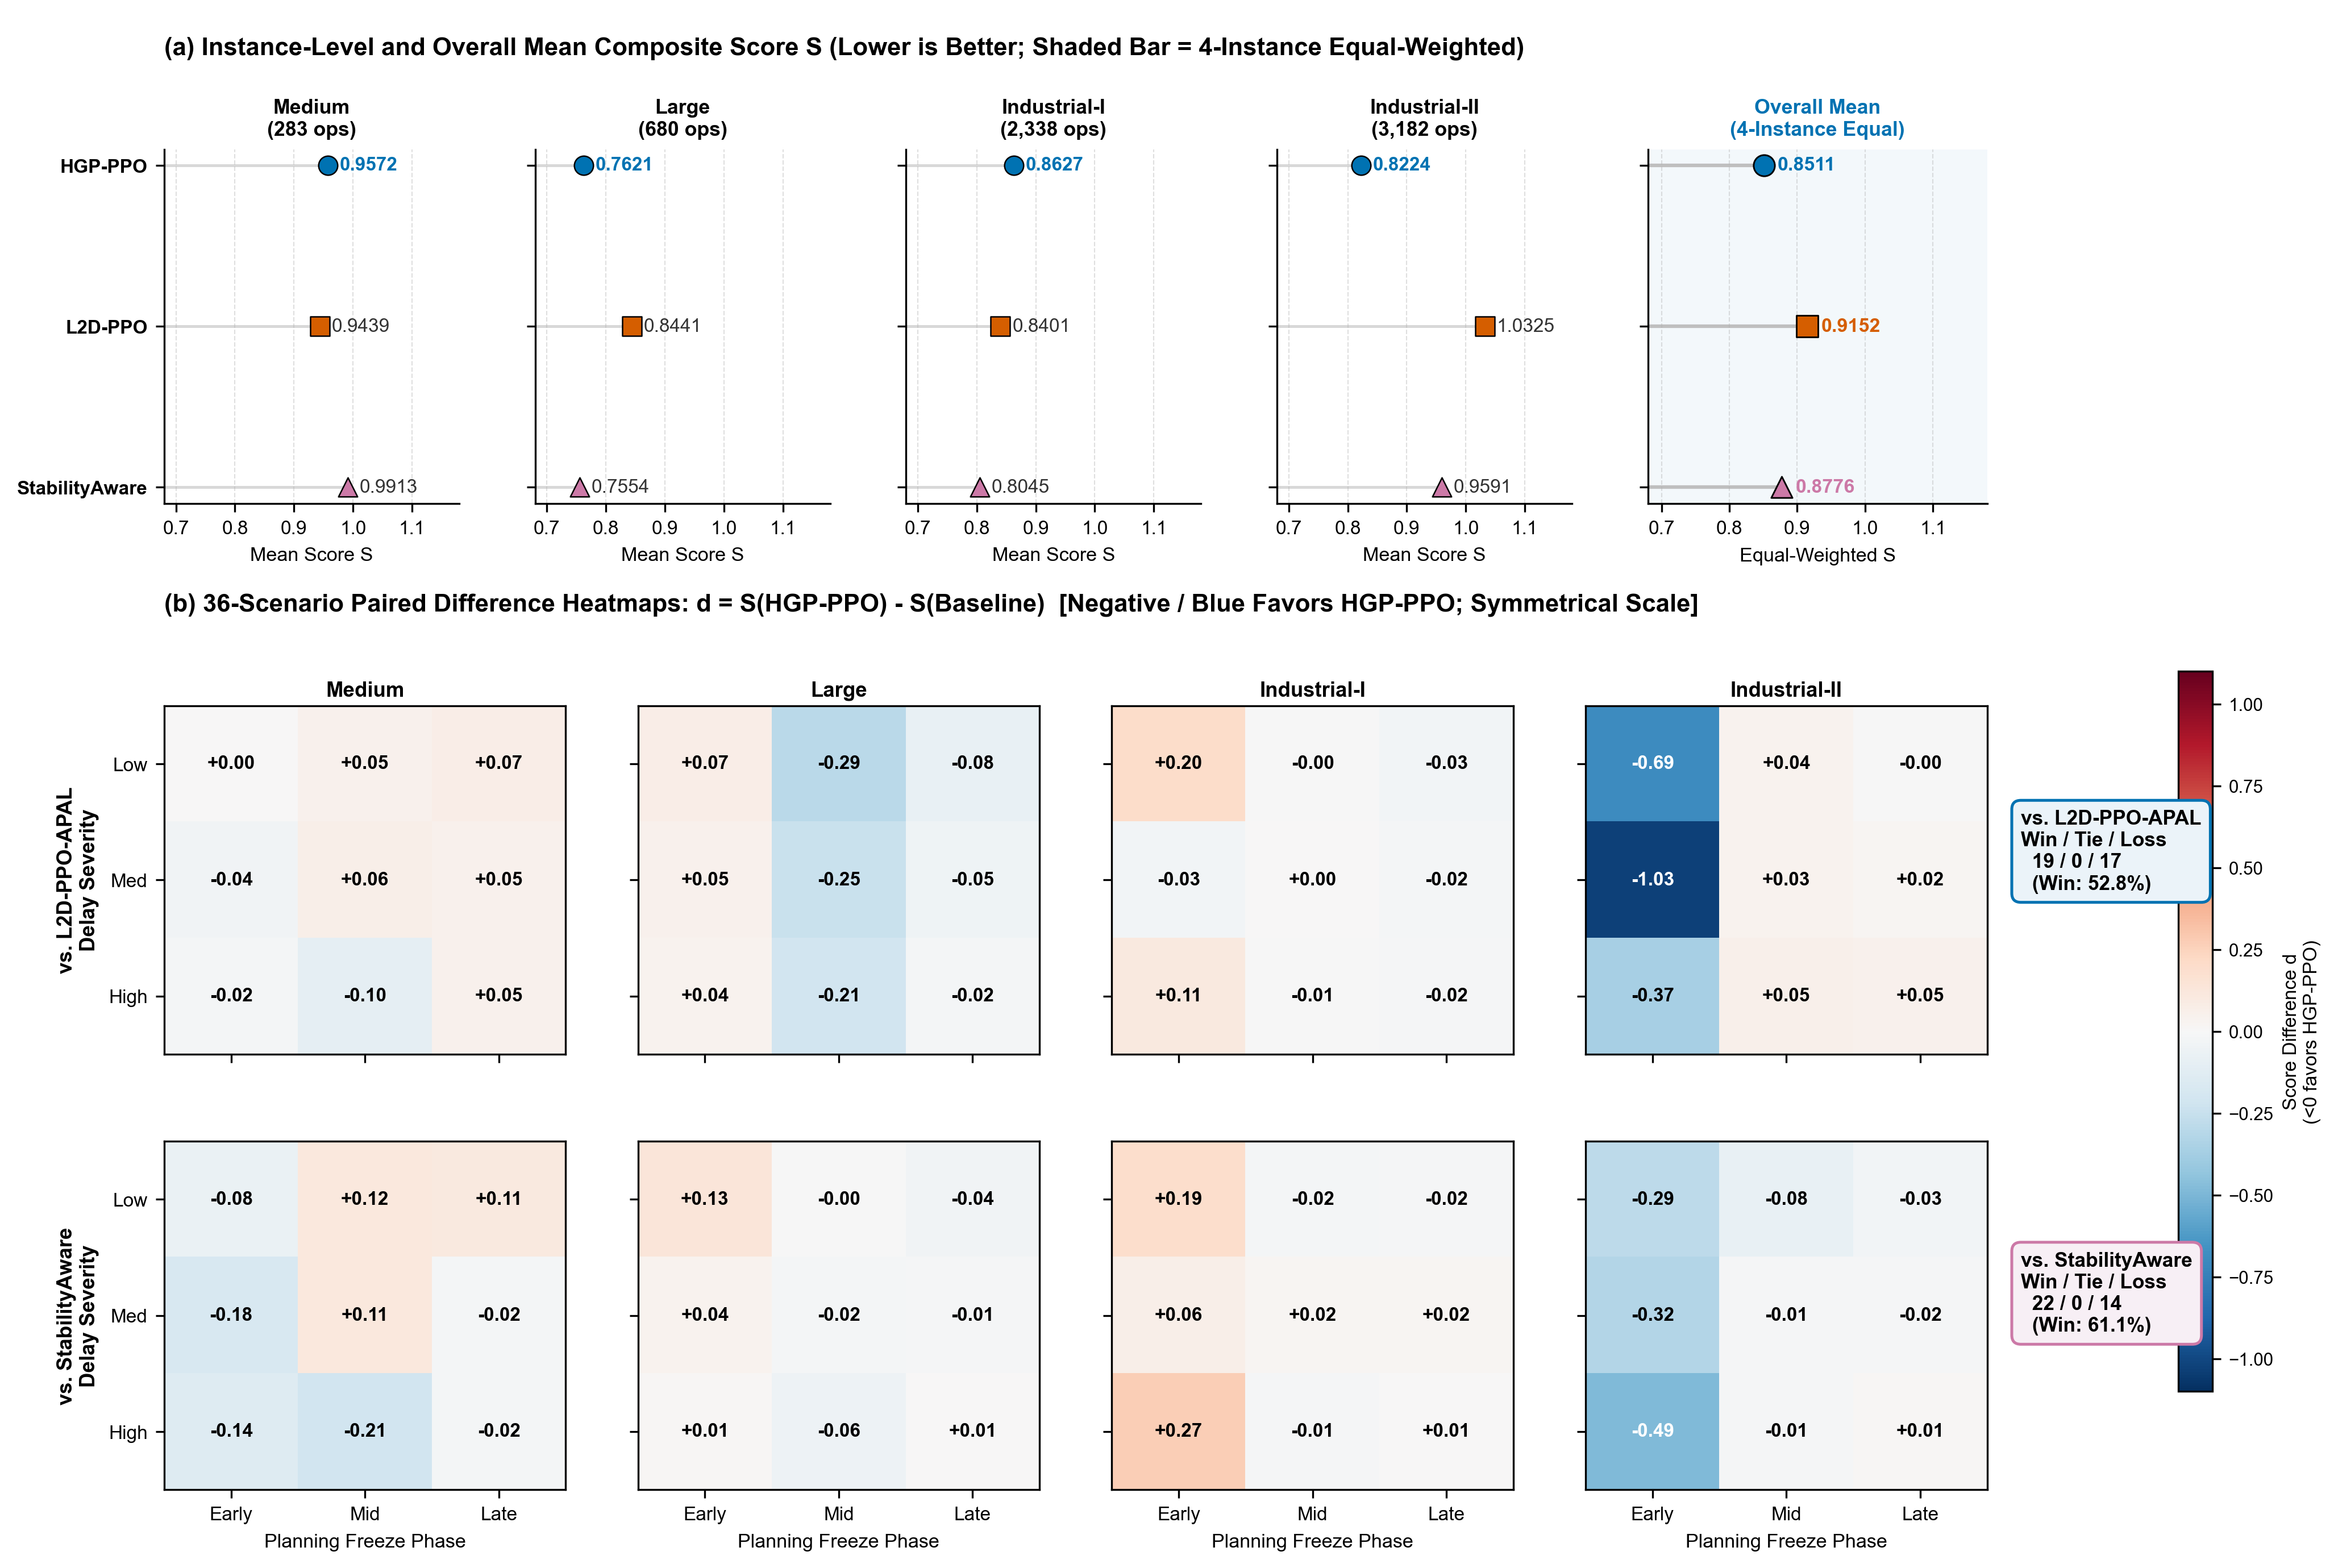
\includegraphics[width=\textwidth,height=0.26\textheight,keepaspectratio]{figures/fig4_reschedule_scenarios_heatmap.png}
\vspace{2pt}
\parbox{\textwidth}{\footnotesize \textbf{图 4　动态物料延误下模板重调度 36 场景配对差值热图与实例级恢复均值点图。} (a) Medium、Large、Industrial-I 与 Industrial-II 四个物理规模实例及四实例等权平均下的综合恢复得分 $S$（越小越好）；(b) 本文方法相对于 L2D-PPO-APAL 和 StabilityAwareRepair 在 36 个扰动场景上的配对得分差值 $d = S_{\mathrm{HGP}} - S_{\mathrm{Baseline}}$ 对称发散热图（蓝色表示本文方法占优，红色表示基准占优），顶部标明两两比较的胜／平／负统计徽章。}
\end{figure*}

\begin{table}[!t]
\centering
\caption{四规模重调度的单场景端到端求解时间（s）}
\label{tab:runtime}
\setlength{\tabcolsep}{4pt}
\renewcommand{\arraystretch}{0.95}
\begin{adjustbox}{max width=\columnwidth}
\begin{tabular}{@{}lrrrr@{}}
\toprule
\textbf{算法名称} & \textbf{Medium} & \textbf{Large} & \textbf{Industrial-I} & \textbf{Industrial-II} \\
\midrule
本文方法 (Proposed HGP-PPO) & \textbf{8.02} & \textbf{12.84} & \textbf{51.91} & \textbf{123.60} \\
Beam\allowbreak{}Search\allowbreak{}Repair & 114.02 & 262.72 & 1787.00 & 3902.89 \\
Iterated\allowbreak{}Greedy\allowbreak{}Repair & 147.17 & 410.42 & 2416.80 & 4202.01 \\
Simulated\allowbreak{}Annealing\allowbreak{}Repair & 292.42 & 676.78 & 3445.39 & 4296.64 \\
\bottomrule
\end{tabular}
\end{adjustbox}
\vspace{2pt}
\par\noindent{\scriptsize 注：时间覆盖构建、推断或搜索、前向分配及校验。本文方法各单元格为 9 个场景均值；搜索方法为 27 条记录单次均值。}\par
\end{table}

\begin{figure}[!t]
\centering
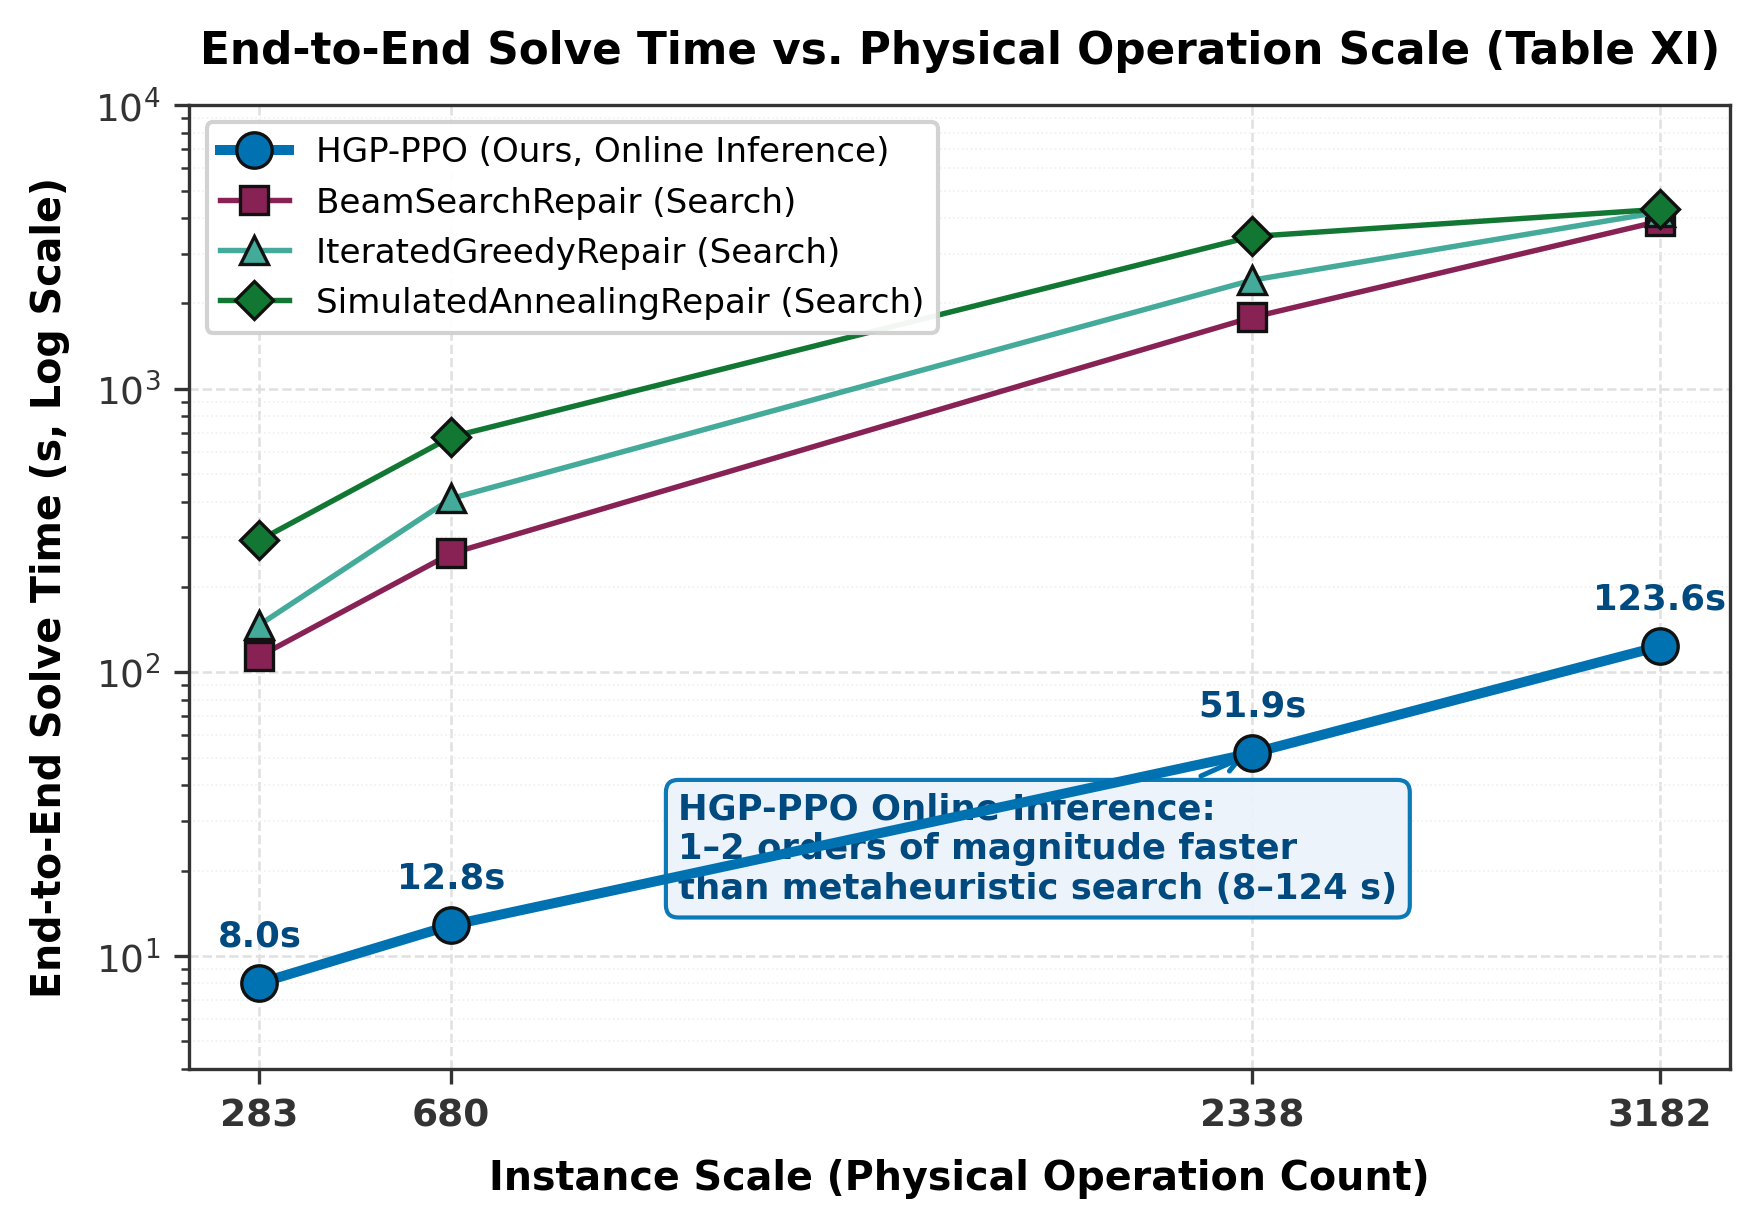
\includegraphics[width=\columnwidth,keepaspectratio]{figures/fig5_runtime_scalability.png}
\vspace{2pt}
\parbox{\columnwidth}{\footnotesize \textbf{图 5　跨物理尺度在线重调度端到端求解耗时与计算扩展性对数对比。} 比较本文方法（神经前向推断）与 Beam Search、Iterated Greedy 及 Simulated Annealing 启发式搜索在 283 至 3182 物理工序规模下的单场景端到端求解时间（秒，对数坐标）。}
\end{figure}

如表 XI 与图 5 所示，逐实例搜索在大规模场景上的耗时呈现急剧增长（在 Industrial-II 规模下单次修复需 3900--4300 s）；而本文方法依托轻量化神经前向推断，在 Industrial-II（3,182 道工序）规模下亦能在约 2 分钟（123.60~s）内完成全线方案修复，较启发式搜索展现出超过 30 倍的计算加速，具备极强的工业级在线实时响应能力。

\section{结论与局限性}\label{sec:conclusions}

本文提出了基于异构图强化学习的飞机脉动装配线联合调度与人员配置方法 HGP-PPO。通过工序---站位---工人的分层条件自回归指针解码器与动态掩码，避免了显式枚举完整团队；内生工人---站位绑定机制协调了人力配置与站位工作负荷。在初始排程中，同一锁定策略无需针对特定实例微调，直接评价于 283 至 3182 道物理工序（Medium, Large, Industrial-I, Industrial-II），展现出强劲的跨规模外推能力与最低的四规模平均完工跨度 902.40~h。在重调度中，扰动环境下训练的策略评价于 36 个锁定物料延误场景，所有测试实例与场景生成的方案均通过模型约束校验，取得更低的平均综合恢复得分并在各稳定性分项间形成权衡，且在 Industrial-II 上的单场景平均端到端修复耗时仅约 2 分钟（123.60~s）。

\textit{局限性与未来工作：}
本文建模面向周期作业模板及其计划级修复。命题~1 确立了固定模板稳态展开的物理可行性；但未确立新旧模板之间瞬态切换的可行性。模型未显式模拟切换过程中的跨架次在制品（WIP）流动与缓冲区拥塞。物料到达延误的更新释放时间假定在重调度触发时已知，标准加工时间假定为确定性。未来工作将拓展至产线瞬态动态仿真、不确定物料到达与加工时间建模，以及工人疲劳与时变工效分析。

\appendices

\section{Worker Pointer 架构、团队状态与候选动态特征}\label{app:worker_pointer}

\textbf{网络结构与部分团队表示。} 对已选成员序列 $\mathbf w_t^{(<r)}$，每个入选工人先由线性层投影为 $\mathbf m_v = \mathbf W_{\mathrm{mem}}\mathbf h_v$。为保证置换不变性，部分团队状态采用 Sum、Mean 与 Max 三路池化特征拼接融合：
\begin{equation}
\begin{aligned}
\mathbf h_{\mathrm{team},t}^{(r)} = \operatorname{LeakyReLU}\Big(\mathbf W_{\mathrm{team}} \Big[ &\sum_{v\in \mathbf w_t^{(<r)}} \mathbf m_v \\
&\Big\|\, \frac{1}{\max(1, r-1)}\sum_{v\in \mathbf w_t^{(<r)}} \mathbf m_v \\
&\Big\|\, \max_{v\in \mathbf w_t^{(<r)}} \mathbf m_v \Big]\Big).
\end{aligned}
\end{equation}
对于首个成员选择步（$r=1$ 且 $\mathbf w_t^{(<1)}=\emptyset$），约定池化结果为零向量 $\mathbf 0\in\mathbb R^d$，退化为零嵌入 $\mathbf h_{\mathrm{team},t}^{(1)}=\mathbf 0$。

查询向量 $\mathbf q_t^{(r)}$ 拼接工序、站位、全局上下文、团队状态、宏观压力、技能消耗比及选人进度后投影：
\begin{equation}
\begin{aligned}
\mathbf q_t^{(r)} = \mathbf W_q\Big[ &\mathbf h_{i_t}\,\|\,\mathbf h_{m_t}\,\|\,\mathbf g_t\,\|\,\mathbf h_{\mathrm{team},t}^{(r)} \\
&\|\,\mathbf P_t\,\|\,\mathbf c_t^{(r)}\,\|\,\mathbf{prog}_t^{(r)}\Big]+\mathbf b_q,
\end{aligned}
\end{equation}
其中全局上下文 $\mathbf g_t = [\mathbf g_M \,\|\, \mathbf g_O \,\|\, \mathbf g_W] \in \mathbb R^{3d}$；宏观压力特征 $\mathbf P_t = [\mathbf P_t^{\mathrm{all}} \,\|\, \mathbf P_t^{\mathrm{near}}] \in \mathbb R^{10}$；技能消耗比向量 $\mathbf c_t^{(r)} = \mathbf C_t^{(r)} / \max(\mathbf S_t^{\mathrm{all}}, \varepsilon_s) \in [0,1]^5$；选人进度向量 $\mathbf{prog}_t^{(r)} = [(r-1)/q_{i_t},\, (q_{i_t}-(r-1))/q_{i_t}]^\top \in [0,1]^2$。

候选工人键向量由工人嵌入、技能压力暴露特征投影后叠加动态项构成：
\begin{equation}
\mathbf k_{w,t}^{(r)} = \mathbf W_k [\mathbf h_w \,\|\, \mathbf e_{w,t}] + \mathbf W_{\mathrm{eft}}\mathbf f_{w,t}^{\mathrm{eft},(r)} + \mathbf W_{\mathrm{sc}}\mu_{w,t}^{(r)}.
\end{equation}
其中 $\mathbf e_{w,t} = [\mathbf H_w \odot \mathbf P_t^{\mathrm{all}} \,\|\, \mathbf H_w \odot \mathbf P_t^{\mathrm{near}}] \in \mathbb R^{10}$。打分层为 $\mathbf v_W^{\top}\tanh(\mathbf q_t^{(r)} + \mathbf k_{w,t}^{(r)})$，非法候选填入 $-\infty$。

\textbf{全局与近端技能压力。} 令 $R_{jk}\in\{0,1\}$ 表示工序 $j$ 是否需要技能 $k$，$H_{wk}\in\{0,1\}$ 表示工人 $w$ 是否具备技能 $k$。令 $\mathcal U_t$ 为未调度物理工序集，$\mathcal R_t$ 为当前就绪工序集：
\begin{align}
D_{k,t}^{\mathrm{all}} &= \sum_{j\in\mathcal U_t}R_{jk}\widetilde p_jq_j, \quad D_{k,t}^{\mathrm{near}} = \sum_{j\in\mathcal R_t}R_{jk}\widetilde p_jq_j, \\
S_{k,t}^{\mathrm{all}} &= \sum_{w\in\mathcal W}H_{wk}, \quad S_{k,t}^{\mathrm{near}} = \sum_{w\in\mathcal W_t^q} H_{wk}\exp\!\left(-\frac{\widetilde a_{w,t}}{\tau_p}\right), \\
P_{k,t}^{h} &= \log\!\left( 1+\frac{D_{k,t}^{h}}{\max(S_{k,t}^{h},\varepsilon_s)} \right), \quad h\in\{\mathrm{all},\mathrm{near}\}.
\end{align}
折减温度设为 $\tau_p=1.0$，平滑常数 $\varepsilon_s=10^{-6}$。

\textbf{动态 EFT。} 加入候选工人 $w$ 后的归一化试探完工量为：
\begin{equation}
\begin{aligned}
\widehat C_{w,t}^{(r)} ={}& \max\!\left(A_t^{(r-1)},\widetilde a_{w,t},\widetilde a_{m_t,t}\right) \\
&+ \frac{\widetilde p_{i_t}q_{i_t}}{\rho^{r-1}\left(E_t^{(r-1)}+\eta_w\right)}, \quad \rho=0.95.
\end{aligned}
\end{equation}
在合法候选工人集合 $\mathcal F_{W,t}^{(r)}$ 上统计最低完工量 $C_{\min,t}^{(r)}$、均值 $\mu_{C,t}^{(r)}$ 与标准差 $\sigma_{C,t}^{(r)}$，动态 EFT 派生特征为：
\begin{align}
\sigma_{C,t}^{(r)} &= \sqrt{\frac{1}{|\mathcal F_{W,t}^{(r)}|} \sum_{u\in\mathcal F_{W,t}^{(r)}} \left(\widehat C_{u,t}^{(r)}-\mu_{C,t}^{(r)}\right)^2}, \\
\mathbf f_{w,t}^{\mathrm{eft},(r)} &= \begin{bmatrix}
\operatorname{clip}\left(\frac{\widehat C_{w,t}^{(r)}-C_{\min,t}^{(r)}}{\widetilde p_{i_t}}, 0, 10\right) \\[6pt]
\operatorname{clip}\left(\frac{\widehat C_{w,t}^{(r)}-\mu_{C,t}^{(r)}}{\max(\sigma_{C,t}^{(r)}, 10^{-6})}, -10, 10\right)
\end{bmatrix}.
\end{align}

\textbf{额外技能边际稀缺度。} 候选工人 $w$ 的额外技能边际稀缺度定义为：
\begin{equation}
\begin{aligned}
\mu_{w,t}^{(r)} = \sum_{k\in\mathcal K} H_{wk}&(1-R_{i_tk}) \Bigg[ \\
&\log\!\left(1 + \frac{D_{k,t}^{\mathrm{all}}}{\max(S_{k,t}^{\mathrm{all}}-C_{k,t}^{(r)}-H_{wk},\varepsilon_s)}\right) \\
&- \log\!\left(1 + \frac{D_{k,t}^{\mathrm{all}}}{\max(S_{k,t}^{\mathrm{all}}-C_{k,t}^{(r)},\varepsilon_s)}\right) \Bigg]_+.
\end{aligned}
\end{equation}
因子 $1-R_{i_tk}$ 排除当前工序所需技能，衡量占用该工人附带其他技能的边际压力增量。

\section{实验复现与统计审计配置}\label{app:reproducibility}

\begin{table}[!t]
\centering
\caption{本文方法的关键复现超参数（Hyperparameters）}
\label{tab:reproducibility}
\setlength{\tabcolsep}{2.5pt}
\renewcommand{\arraystretch}{0.92}
\begin{adjustbox}{max width=\columnwidth}
\begin{tabular}{@{}llp{4.2cm}@{}}
\toprule
\textbf{类别} & \textbf{参数项} & \textbf{正式设定} \\
\midrule
数据规模 & 训练集／验证集／测试集 & 24／6／4 个实例 \\
扰动场景 & 验证集／测试集 & 54／36；每实例 9 个固定场景 \\
网络架构 & 节点嵌入与 GATv2 & 5 层 GATv2，4 头，隐藏维 $d=128$ \\
模型规模 & 可训练参数量 & 约 11.2 M \\
PPO & 学习率／$\gamma$／GAE $\lambda$ & $1.0\times10^{-4}$／0.999／0.9 \\
PPO & 更新轮数／裁剪范围 & 2／0.20 线性衰减至 0.10 \\
数值处理 & 差分放大／裁剪／全局缩放 & 100／$[-50,50]$／0.005 \\
损失正则 & 价值系数 $c_V$／熵系数 $c_H$ & 0.5／$2.0\times10^{-4}\to 5.0\times10^{-5}$ \\
优化配置 & 优化器／权重衰减 & ScheduleFree AdamW／$1.0\times10^{-4}$ \\
梯度控制 & Actor／Critic 梯度范数上限 & 0.5／0.05 \\
重调度采样 & 批量／并行环境／累积步数 & 64 或 128／4／4 \\
数值精度 & 训练精度 & BF16 混合精度 \\
训练预算 & 初始排程／重调度 & 60 轮／120 轮（双阶段） \\
主评价解码 & 解码规则／温度 & masked argmax／0 \\
\bottomrule
\end{tabular}
\end{adjustbox}
\end{table}

\textbf{统计度量指标定义}：
1)~\textit{截断均值（IQM）}：去除升序中最低 25\% 与最高 25\% 极端值后中间 50\% 样本的算术均值。
2)~\textit{平均相对偏差（ARD）}：对方法 $m$ 在场景集 $\mathcal S$（$|\mathcal S|=36$）上：$\mathrm{ARD}_m = \frac{1}{|\mathcal S|}\sum_{s\in\mathcal S} \frac{S_{ms}-S_s^*}{S_s^*}\times100\%$，其中 $S_s^*=\min_k S_{ks}$ 为所有参评合法方法在场景 $s$ 中观测到的最优得分。
3)~\textit{配对秩双列相关系数（$r_{\mathrm{rb}}$）}：Wilcoxon 符号秩检验的配对无参数效应量：$r_{\mathrm{rb}}=(W^+-W^-)/(W^++W^-)\in[-1,1]$。

\begin{thebibliography}{30}
\bibitem{fang2021}
S.~Fang, M.~Liu, G.~Xian, et~al., ``Aircraft moving assembly line: Pulsating and continuous,'' \textit{Aeronaut. Manuf. Technol.}, vol. 64, no. 16, pp. 40--50, 2021.
\bibitem{bao2023}
Z.~Bao, L.~Chen, and K.~Qiu, ``An aircraft final assembly line balancing problem considering resource constraints and parallel task scheduling,'' \textit{Comput. Ind. Eng.}, vol. 182, p. 109436, 2023.
\bibitem{wang2024}
D.~Wang, F.~Qiao, L.~Guan, et~al., ``Human--machine collaborative optimization method for dynamic worker allocation in aircraft final assembly lines,'' \textit{Comput. Ind. Eng.}, vol. 194, p. 110370, 2024.
\bibitem{lu2019}
Z.~Lu, Y.~Ren, L.~Wang, et~al., ``A resource investment problem based on project splitting with time windows for aircraft moving assembly line,'' \textit{Comput. Ind. Eng.}, vol. 135, pp. 568--581, 2019.
\bibitem{becker2006}
C.~Becker and A.~Scholl, ``A survey on problems and methods in generalized assembly line balancing,'' \textit{Eur. J. Oper. Res.}, vol. 168, no. 3, pp. 694--715, 2006.
\bibitem{boysen2007}
N.~Boysen, M.~Fliedner, and A.~Scholl, ``A classification of assembly line balancing problems,'' \textit{Eur. J. Oper. Res.}, vol. 183, no. 2, pp. 674--693, 2007.
\bibitem{vieira2003}
G.~E.~Vieira, J.~W.~Herrmann, and E.~Lin, ``Rescheduling manufacturing systems: A framework of strategies, policies, and methods,'' \textit{J. Sched.}, vol. 6, no. 1, pp. 39--62, 2003.
\bibitem{hu2024}
J.-H.~Hu, J.-Y.~Zhu, Y.-N.~Sun, et~al., ``Network-based two-stage robust scheduling strategy for the aircraft assembly system with uncertain duration,'' \textit{Comput. Ind. Eng.}, vol. 188, p. 109911, 2024.
\bibitem{battaia2013}
O.~Batta\"ia and A.~Dolgui, ``A taxonomy of line balancing problems and their solution approaches,'' \textit{Int. J. Prod. Econ.}, vol. 142, no. 2, pp. 259--277, 2013.
\bibitem{bao2023b}
Z.~Bao, L.~Chen, and K.~Qiu, ``A surrogate-assisted heuristic approach for the joint optimization of resource allocation and scheduling of an aircraft final assembly line,'' \textit{J. Manuf. Syst.}, vol. 70, pp. 99--112, 2023.
\bibitem{fang2021flexible}
P.~Fang, J.-J.~Yang, Y.~Jiang, et~al., ``Flexible worker allocation in aircraft final assembly line using multiobjective evolutionary algorithms,'' \textit{IEEE Trans. Ind. Informat.}, vol. 17, no. 11, pp. 7468--7478, 2021.
\bibitem{liu2025}
M.~Liu, L.~Li, X.~Liu, et~al., ``A multi-pass heuristic for multi-skilled worker scheduling in aircraft final assembly line with variable duration,'' \textit{J. Syst. Eng. Electron.}, vol. 36, no. 6, pp. 1532--1547, 2025.
\bibitem{wen2026}
X.~Wen, H.~Liu, X.~Zhang, et~al., ``A Q-learning improved particle swarm optimization for aircraft pulsating assembly line scheduling problem considering skilled operator allocation,'' \textit{Comput. Mater. Contin.}, vol. 86, no. 1, pp. 1--27, 2026.
\bibitem{cappart2023}
Q.~Cappart, D.~Ch\'etelat, E.~B.~Khalil, et~al., ``Combinatorial optimization and reasoning with graph neural networks,'' \textit{J. Mach. Learn. Res.}, vol. 24, no. 130, pp. 1--61, 2023.
\bibitem{zhang2020}
C.~Zhang, W.~Song, Z.~Cao, et~al., ``Learning to dispatch for job shop scheduling via deep reinforcement learning,'' in \textit{Adv. Neural Inf. Process. Syst. (NeurIPS)}, vol. 33, 2020, pp. 1621--1632.
\bibitem{park2021}
J.~Park, J.~Chun, S.~H.~Kim, et~al., ``Learning to schedule job-shop problems: Representation and policy learning using graph neural network and reinforcement learning,'' \textit{Int. J. Prod. Res.}, vol. 59, no. 11, pp. 3342--3359, 2021.
\bibitem{wang2024flexible}
R.~Wang, G.~Wang, J.~Sun, F.~Deng, and J.~Chen, ``Flexible job shop scheduling via dual attention network-based reinforcement learning,'' \textit{IEEE Trans. Neural Netw. Learn. Syst.}, vol. 35, no. 3, pp. 3091--3102, 2024.
\bibitem{ai2025}
J.~Ai, F.~Qiao, J.~Liu, et~al., ``A graph-enhanced deep-reinforcement learning approach for the aircraft pulse assembly line balancing problem,'' in \textit{Proc. 2025 China Autom. Congr. (CAC)}, 2025, pp. 6623--6628.
\bibitem{wen2026b}
X.~Wen, H.~Zhang, W.~Yang, et~al., ``Research on a worker skill level-aware pulsating assembly scheduling method for aircraft based on the GIN-PPO algorithm,'' \textit{Comput. Ind. Eng.}, vol. 218, p. 112135, 2026.
\bibitem{vonder2007}
S.~Van~de~Vonder, E.~Demeulemeester, and W.~Herroelen, ``A classification of predictive-reactive project scheduling procedures,'' \textit{J. Sched.}, vol. 10, no. 3, pp. 195--207, 2007.
\bibitem{zhu2021}
H.~Zhu, Z.~Lu, C.~Lu, and Y.~Ren, ``A reactive scheduling method for disturbances in aircraft moving assembly line,'' \textit{Int. J. Prod. Res.}, vol. 59, no. 15, pp. 4756--4772, 2021.
\bibitem{chen2026}
B.~Chen, J.~Zhang, X.~Luo, et~al., ``A multi-agent graph attention deep reinforcement learning method for aircraft assembly dynamic scheduling,'' \textit{Adv. Eng. Inform.}, vol. 68, p. 104565, 2026.
\bibitem{brody2022}
S.~Brody, U.~Alon, and E.~Yahav, ``How attentive are graph attention networks?'' in \textit{Proc. Int. Conf. Learn. Represent. (ICLR)}, 2022.
\bibitem{schulman2016}
J.~Schulman, P.~Moritz, S.~Levine, et~al., ``High-dimensional continuous control using generalized advantage estimation,'' in \textit{Proc. Int. Conf. Learn. Represent. (ICLR)}, 2016.
\bibitem{schulman2017}
J.~Schulman, F.~Wolski, P.~Dhariwal, et~al., ``Proximal policy optimization algorithms,'' \textit{arXiv preprint arXiv:1707.06347}, 2017.
\bibitem{smith1956}
W.~E.~Smith, ``Various optimizers for single-stage production,'' \textit{Nav. Res. Logist. Q.}, vol. 3, no. 1--2, pp. 59--66, 1956.
\bibitem{kelley1961}
J.~E.~Kelley, Jr., ``Critical-path planning and scheduling: Mathematical basis,'' \textit{Oper. Res.}, vol. 9, no. 3, pp. 296--320, 1961.
\bibitem{ow1988}
P.~S.~Ow and T.~E.~Morton, ``Filtered beam search in scheduling,'' \textit{Int. J. Prod. Res.}, vol. 26, no. 1, pp. 35--62, 1988.
\bibitem{ruiz2007}
R.~Ruiz and T.~St\"utzle, ``A simple and effective iterated greedy algorithm for the permutation flowshop scheduling problem,'' \textit{Eur. J. Oper. Res.}, vol. 177, no. 3, pp. 2033--2049, 2007.
\bibitem{kirkpatrick1983}
S.~Kirkpatrick, C.~D.~Gelatt, and M.~P.~Vecchi, ``Optimization by simulated annealing,'' \textit{Science}, vol. 220, no. 4598, pp. 671--680, 1983.
\end{thebibliography}

\end{document}
